%%%%%%%%%%%%%%%%%%%%%%%%%%%%
%% IHEID CHAPTER TEMPLATE %%
%%%%%%%%%%%%%%%%%%%%%%%%%%%%

%%%% PAGE LAYOUT
% Pass this in from YAML
\documentclass[a4paper, oneside]{report}
\usepackage[includehead,hmargin={3.1cm, 3.1cm}, vmargin={2.5cm,2.7cm}, headsep=.8cm,footskip=1.2cm]{geometry}

\usepackage{fancyhdr}
\setlength{\headheight}{15pt}
\fancyhf{} % clear the header and footers
\pagestyle{fancy}
\renewcommand{\chaptermark}[1]{\markboth{\thechapter. #1}{\thechapter. #1}}
\renewcommand{\sectionmark}[1]{\markright{\thesection. #1}} 
\renewcommand{\headrulewidth}{0pt}
\fancyhead[LO]{\emph{\leftmark}}

\fancypagestyle{plain}{\fancyhf{}\fancyfoot[C]{\emph{\thepage}}}

% This adds a "DRAFT" footer to every normal page.  (The first page of each chapter is not a "normal" page.)
\fancyfoot[C]{\emph{DRAFT: \today}}
\fancyfoot[R]{\emph{\thepage}}

%%%%% FONTS
\RequirePackage[T1]{fontenc} % requires XeLatex or LuaTex (remove to use pdfLaTex)
%\RequirePackage[utf8]{inputenc} % ignored when using XeLaTex or LuaTex (uncomment when using pdfLaTex)
\RequirePackage{microtype} % this makes fonts almost imperceptibly smoother
\RequirePackage{fontspec} % requires XeLatex or LuaTex (remove to use pdfLaTex)
% For the headings we will use Helvetica
\RequirePackage{helvet}
\usepackage[immediate]{silence}
\WarningFilter[temp]{latex}{Command} % silence the warning
\usepackage{sectsty}
\DeactivateWarningFilters[temp] % So nothing unrelated gets silenced
\allsectionsfont{\sffamily}
% For the main text and equations we will use Baskerville and Palatino
\RequirePackage{mathpazo}
\RequirePackage{baskervald}
% For formatting code or package names, we will use Lucida Console
\RequirePackage{zi4}
% Enable strikethrough
\usepackage[normalem]{ulem}

% This highlights (in blue) corrections marked with (for words) \mccorrect{blah} or (for whole
% paragraphs) \begin{mccorrection} . . . \end{mccorrection}.  This can be useful for sending a PDF of
% your corrected thesis to your examiners for review.  Turn it off, and the blue disappears.
% 
% UL 30 Nov 2018 pandoc puts lists in 'tightlist' command when no space between bullet points in Rmd file
\providecommand{\tightlist}{%
  \setlength{\itemsep}{0pt}\setlength{\parskip}{0pt}}
 
%UL 15 Oct 2019, enable link highlighting to be turned off from YAML
% \usepackage[dvipsnames]{color}
% \usepackage[colorlinks=true,pdfpagelabels,hidelinks=false]{hyperref}
\RequirePackage[colorlinks=true,linkcolor=red,
citecolor=red,filecolor=red,urlcolor=black]{hyperref} % uses IHEID red for external links
% \hypersetup{citecolor=red}

%%%%% BIBLIOGRAPHY SETUP
% Note that your bibliography will require some tweaking depending on your department, preferred format, etc.
% The options included below are just very basic "sciencey" and "humanitiesey" options to get started.
% If you've not used LaTeX before, I recommend reading a little about biblatex/biber and getting started with it.
% If you're already a LaTeX pro and are used to natbib or something, modify as necessary.
% Either way, you'll have to choose and configure an appropriate bibliography format...

% The science-type option: numerical in-text citation with references in order of appearance.
% \usepackage[style=numeric-comp, sorting=none, backend=biber, doi=false, isbn=false]{biblatex}
% \newcommand*{\bibtitle}{References}

% The humanities-type option: author-year in-text citation with an alphabetical works cited.
% \usepackage[style=authoryear, sorting=nyt, backend=biber, maxcitenames=2, useprefix, doi=false, isbn=false]{biblatex}
% \newcommand*{\bibtitle}{Works Cited}

%UL 3 Dec 2018: set this from YAML in index.Rmd
% % \usepackage[style=numeric-comp, sorting=none, backend=biber, doi=, isbn=false]{biblatex}
% \newcommand*{\bibtitle}{References}
% 
% This makes the bibliography left-aligned (not 'justified') and slightly smaller font.
% \renewcommand*{\bibfont}{\raggedright\small}

% Change this to the name of your .bib file (usually exported from a citation manager like Zotero or EndNote).
% \addbibresource{bib/references.bib}

% Uncomment this if you want equation numbers per section (2.3.12), instead of per chapter (2.18):
%\numberwithin{equation}{subsection}

\newlength{\cslhangindent}
\setlength{\cslhangindent}{1.5em}
\newenvironment{cslreferences}%
  {\setlength{\parindent}{0pt}%
  \everypar{\setlength{\hangindent}{\cslhangindent}}\ignorespaces}%
  {\par}
  
\usepackage{color}
\usepackage{fancyvrb}
\newcommand{\VerbBar}{|}
\newcommand{\VERB}{\Verb[commandchars=\\\{\}]}
\DefineVerbatimEnvironment{Highlighting}{Verbatim}{commandchars=\\\{\}}
% Add ',fontsize=\small' for more characters per line
\usepackage{framed}
\definecolor{shadecolor}{RGB}{248,248,248}
\newenvironment{Shaded}{\begin{snugshade}}{\end{snugshade}}
\newcommand{\AlertTok}[1]{\textcolor[rgb]{0.94,0.16,0.16}{#1}}
\newcommand{\AnnotationTok}[1]{\textcolor[rgb]{0.56,0.35,0.01}{\textbf{\textit{#1}}}}
\newcommand{\AttributeTok}[1]{\textcolor[rgb]{0.77,0.63,0.00}{#1}}
\newcommand{\BaseNTok}[1]{\textcolor[rgb]{0.00,0.00,0.81}{#1}}
\newcommand{\BuiltInTok}[1]{#1}
\newcommand{\CharTok}[1]{\textcolor[rgb]{0.31,0.60,0.02}{#1}}
\newcommand{\CommentTok}[1]{\textcolor[rgb]{0.56,0.35,0.01}{\textit{#1}}}
\newcommand{\CommentVarTok}[1]{\textcolor[rgb]{0.56,0.35,0.01}{\textbf{\textit{#1}}}}
\newcommand{\ConstantTok}[1]{\textcolor[rgb]{0.00,0.00,0.00}{#1}}
\newcommand{\ControlFlowTok}[1]{\textcolor[rgb]{0.13,0.29,0.53}{\textbf{#1}}}
\newcommand{\DataTypeTok}[1]{\textcolor[rgb]{0.13,0.29,0.53}{#1}}
\newcommand{\DecValTok}[1]{\textcolor[rgb]{0.00,0.00,0.81}{#1}}
\newcommand{\DocumentationTok}[1]{\textcolor[rgb]{0.56,0.35,0.01}{\textbf{\textit{#1}}}}
\newcommand{\ErrorTok}[1]{\textcolor[rgb]{0.64,0.00,0.00}{\textbf{#1}}}
\newcommand{\ExtensionTok}[1]{#1}
\newcommand{\FloatTok}[1]{\textcolor[rgb]{0.00,0.00,0.81}{#1}}
\newcommand{\FunctionTok}[1]{\textcolor[rgb]{0.00,0.00,0.00}{#1}}
\newcommand{\ImportTok}[1]{#1}
\newcommand{\InformationTok}[1]{\textcolor[rgb]{0.56,0.35,0.01}{\textbf{\textit{#1}}}}
\newcommand{\KeywordTok}[1]{\textcolor[rgb]{0.13,0.29,0.53}{\textbf{#1}}}
\newcommand{\NormalTok}[1]{#1}
\newcommand{\OperatorTok}[1]{\textcolor[rgb]{0.81,0.36,0.00}{\textbf{#1}}}
\newcommand{\OtherTok}[1]{\textcolor[rgb]{0.56,0.35,0.01}{#1}}
\newcommand{\PreprocessorTok}[1]{\textcolor[rgb]{0.56,0.35,0.01}{\textit{#1}}}
\newcommand{\RegionMarkerTok}[1]{#1}
\newcommand{\SpecialCharTok}[1]{\textcolor[rgb]{0.00,0.00,0.00}{#1}}
\newcommand{\SpecialStringTok}[1]{\textcolor[rgb]{0.31,0.60,0.02}{#1}}
\newcommand{\StringTok}[1]{\textcolor[rgb]{0.31,0.60,0.02}{#1}}
\newcommand{\VariableTok}[1]{\textcolor[rgb]{0.00,0.00,0.00}{#1}}
\newcommand{\VerbatimStringTok}[1]{\textcolor[rgb]{0.31,0.60,0.02}{#1}}
\newcommand{\WarningTok}[1]{\textcolor[rgb]{0.56,0.35,0.01}{\textbf{\textit{#1}}}}
%UL 2 Dec 2018 add a bit of white space before and after code blocks
\renewenvironment{Shaded}
{
  \vspace{4pt}%
  \begin{snugshade}%
}{%
  \end{snugshade}%
  \vspace{4pt}%
}

%%%%% THESIS / TITLE PAGE INFORMATION
% Everybody needs to complete the following:
\title{Conclusion}
\author{Chin Man KWAN}

% JEM: Lengths for single spacing (ie separate abstract, captions), front matter (abstract,
%   acknowledgements, table of contents, etc), and main body text.
\newlength{\singlebaselineskip}
\newlength{\frontmatterbaselineskip}
\newlength{\textbaselineskip}

\setlength{\singlebaselineskip}{\baselineskip}
\setlength{\frontmatterbaselineskip}{17pt plus1pt minus1pt}
\setlength{\textbaselineskip}{22pt plus2pt}

%
% Environments
%

% Managing minitoc for chapters
% \usepackage[nohints,tight]{minitoc} 
% 	\setcounter{minitocdepth}{2} 
% 	% Generates mini tables of contents per chapter
% 	
% % JEM: The following fixes minitoc to not be multiple-spaced.
% \makeatletter
% \let\oldmtc@verse\mtc@verse
% \renewcommand{\mtc@verse}[1]{\oldmtc@verse{#1}\setlength{\baselineskip}{\z@}}
% \makeatother
	
% For the abbreviations
\usepackage{enumitem}
\newlist{abbrv}{itemize}{1}
\setlist[abbrv,1]{label=,labelwidth=1in,align=parleft,itemsep=0.1\baselineskip,leftmargin=!}

\usepackage{nicefrac}
\usepackage{amsmath}
\usepackage{amssymb}
\usepackage{textcomp}

\usepackage{longtable} 
	% Allows tables to span multiple pages (this package must be called before hyperref)

\usepackage[font=small,labelfont=bf]{caption} 
	% Nicer captions

\usepackage{multicol,multirow,array} 
	% Used to make multiple columns for the indices and for creating columns that span multiple rows in tables

\usepackage{rotating} 
	% To allow tables in landscape mode

\usepackage{booktabs} 
	% For better looking tables

\usepackage{pdfpages} 
	% Allows multi-page pdfs to be inserted as graphics
	
\usepackage{graphicx}
\graphicspath{{../figures/}{_bookdown_files/}}

\usepackage{xfrac}

%%%%%%%%%%%%%%%%%%%%%%%%%%%
%% ACTUAL DOCUMENT HERE  %%
%%%%%%%%%%%%%%%%%%%%%%%%%%%
\begin{document}

\maketitle



\tableofcontents

%%%%% CHOOSE YOUR LINE SPACING HERE
% This is the official option.  Use it for your submission copy and library copy:
\setlength{\textbaselineskip}{22pt plus2pt}
% This is closer spacing (about 1.5-spaced) that you might prefer for your personal copies:
%\setlength{\textbaselineskip}{18pt plus2pt minus1pt}

% You can set the spacing here for the roman-numbered pages (acknowledgements, table of contents, etc.)
\setlength{\frontmatterbaselineskip}{17pt plus1pt minus1pt}

% UL: You can set the general paragraph spacing here - I've set it to 2pt (was 0) so
% it's less claustrophobic
\setlength{\parskip}{2pt plus 1pt}

% Leave this line alone; it gets things started for the real document.
\setlength{\baselineskip}{\textbaselineskip}

%%%%% CHAPTERS
% Add or remove any chapters you'd like here, by file name (excluding '.tex'):
\flushbottom

% all your chapters and appendices will appear here
\hypertarget{examiner-aragorn-ii-elessar-only-required-if-phd-otherwise-delete-or-comment-out}{%
\chapter{examiner: Aragorn II Elessar \# only required if PhD; otherwise
delete or comment
out}\label{examiner-aragorn-ii-elessar-only-required-if-phd-otherwise-delete-or-comment-out}}

Placeholder

\hypertarget{metadata}{%
\section{Metadata}\label{metadata}}

\hypertarget{front-matter}{%
\section{Front Matter}\label{front-matter}}

\hypertarget{bibliography}{%
\section{Bibliography}\label{bibliography}}

\hypertarget{pdf-formatting}{%
\section{PDF Formatting}\label{pdf-formatting}}

\hypertarget{output-options}{%
\section{Output Options}\label{output-options}}

\hypertarget{intro}{%
\chapter{Introduction}\label{intro}}

Placeholder

\hypertarget{theory}{%
\chapter{Literature Review}\label{theory}}

Placeholder

\hypertarget{theories}{%
\section{Theories}\label{theories}}

\hypertarget{what-is-national-identity}{%
\subsection{What is national
identity?}\label{what-is-national-identity}}

\hypertarget{impact-of-conceptions-of-national-identity-on-attitudes-towards-immigrants}{%
\subsection{Impact of conceptions of national identity on attitudes
towards
immigrants}\label{impact-of-conceptions-of-national-identity-on-attitudes-towards-immigrants}}

\hypertarget{chineseness-in-hong-kong}{%
\subsection{Chineseness in Hong Kong}\label{chineseness-in-hong-kong}}

\hypertarget{empirics}{%
\section{Empirics}\label{empirics}}

\hypertarget{how-do-different-political-camps-in-hong-kong-perceive-national-identity}{%
\subsection{How do different political camps in Hong Kong perceive
national
identity?}\label{how-do-different-political-camps-in-hong-kong-perceive-national-identity}}

\hypertarget{the-pro-beijing-camp}{%
\subsubsection{The pro-Beijing camp}\label{the-pro-beijing-camp}}

\hypertarget{the-pro-democracy-camp-or-pan-democrats}{%
\subsubsection{The pro-Democracy camp (or
pan-democrats)}\label{the-pro-democracy-camp-or-pan-democrats}}

\hypertarget{the-localist-camp}{%
\subsubsection{The localist camp}\label{the-localist-camp}}

\hypertarget{asylum-seekers-in-hong-kong}{%
\subsection{Asylum seekers in Hong
Kong}\label{asylum-seekers-in-hong-kong}}

\hypertarget{hong-kongs-policy-regime}{%
\subsubsection{Hong Kong's policy
regime}\label{hong-kongs-policy-regime}}

\hypertarget{responses-by-political-camps}{%
\subsubsection{Responses by political
camps}\label{responses-by-political-camps}}

\hypertarget{methods}{%
\chapter{Methods}\label{methods}}

Placeholder

\hypertarget{hypotheses}{%
\section{Hypotheses}\label{hypotheses}}

\hypertarget{data-collection}{%
\section{Data collection}\label{data-collection}}

\hypertarget{modelling}{%
\section{Modelling}\label{modelling}}

\hypertarget{operationalisation}{%
\section{Operationalisation}\label{operationalisation}}

\hypertarget{main-independent-variable}{%
\subsection{Main independent variable}\label{main-independent-variable}}

\hypertarget{dependent-variable}{%
\subsection{Dependent variable}\label{dependent-variable}}

\hypertarget{control-variables}{%
\subsection{Control variables}\label{control-variables}}

\setcounter{chapter}{3}

\begin{Shaded}
\begin{Highlighting}[]
\FunctionTok{library}\NormalTok{(reticulate)}
\end{Highlighting}
\end{Shaded}

\begin{Shaded}
\begin{Highlighting}[]
\ImportTok{import}\NormalTok{ warnings}
\ImportTok{import}\NormalTok{ numpy }\ImportTok{as}\NormalTok{ np}
\ImportTok{import}\NormalTok{ pandas }\ImportTok{as}\NormalTok{ pd}
\ImportTok{import}\NormalTok{ matplotlib.pyplot }\ImportTok{as}\NormalTok{ plt}
\ImportTok{import}\NormalTok{ seaborn }\ImportTok{as}\NormalTok{ sns}
\ImportTok{import}\NormalTok{ jieba}
\ImportTok{import}\NormalTok{ zhon.hanzi}
\ImportTok{import}\NormalTok{ re}
\ImportTok{from}\NormalTok{ itertools }\ImportTok{import}\NormalTok{ chain}

\CommentTok{\# Setting options for display and random seed}
\NormalTok{np.random.seed(}\DecValTok{1}\NormalTok{)}
\NormalTok{pd.set\_option(}\StringTok{\textquotesingle{}display.max\_columns\textquotesingle{}}\NormalTok{, }\VariableTok{None}\NormalTok{)}
\NormalTok{sns.set\_theme(context}\OperatorTok{=}\StringTok{\textquotesingle{}paper\textquotesingle{}}\NormalTok{)}
\NormalTok{warnings.filterwarnings(category}\OperatorTok{=}\PreprocessorTok{FutureWarning}\NormalTok{, action }\OperatorTok{=} \StringTok{\textquotesingle{}ignore\textquotesingle{}}\NormalTok{)}
\end{Highlighting}
\end{Shaded}

\begin{Shaded}
\begin{Highlighting}[]
\NormalTok{news\_df }\OperatorTok{=}\NormalTok{ pd.read\_csv(}\StringTok{"Coding/asylum\_seekers\_articles\_final.csv"}\NormalTok{)}
\NormalTok{num\_of\_articles }\OperatorTok{=}\NormalTok{ news\_df.shape[}\DecValTok{0}\NormalTok{]}
\NormalTok{num\_of\_newspapers }\OperatorTok{=}\NormalTok{ news\_df.Newspaper.nunique()}
\end{Highlighting}
\end{Shaded}

\hypertarget{results}{%
\chapter{Results}\label{results}}

After searching for articles which contain at least one of the keywords
and are relevant to asylum seekers residing in Hong Kong, there were in
total 557 articles published in 2019 by 16 newspapers. In this section,
I will first explore the data set preliminarily, and then move onto
sentiment analysis with machine learning models to find out whether the
political camp of media outlets is associated with the polarity of the
news articles towards asylum seekers.

\hypertarget{exploratory-data-analysis-eda}{%
\section{Exploratory data analysis
(EDA)}\label{exploratory-data-analysis-eda}}

\hypertarget{how-does-the-number-of-news-articles-vary-by-political-camps-and-month}{%
\subsection{How does the number of news articles vary by political camps
and
month?}\label{how-does-the-number-of-news-articles-vary-by-political-camps-and-month}}

Starting with the number of articles by media outlets as shown in the
left plot of figure 4.1, consistent with the study by Ng, Choi, and Chan
(\protect\hyperlink{ref-ngFramingIssueAsylum2019}{2019}), Oriental Daily
News continues to be the media outlet covering the most frequently on
asylum seekers with 384 (or 68.94\%) articles throughout 2019. By
contrast, the second-most frequent publisher \emph{Sing Tao Daily} only
had 45 entries (or 8.08\%) of the total number of articles published.
Each of the other newspaper outlets only constituted to a small portion
of news articles about non-refoulement claimants in 2019. Therefore, the
issue of asylum seekers in Hong Kong still appeared to be the most
salient for Oriental Daily News by 2019, evidenced by its unmatched
volume of articles related to this topic vis-a-vis other media outlets.

On a higher level of political stance, the right plot of figure 4.1
indicates that largely due to the huge volume of articles by Oriental
Daily News, the pro-Beijing camp dominated the coverage of asylum
seekers in Hong Kong in 2019. Meanwhile, both neutral and pro-democracy
newspaper outlets published similar amounts of articles throughout 2019,
and both camps constituted to small proportions of the share of articles
during the year. Even if we omitted the sheer volume of articles
published by Oriental Daily News, the pro-Beijing media would still have
173 articles published altogether which was still considerably more than
the quantity of articles by neutral and pro-democracy media outlets.

\begin{Shaded}
\begin{Highlighting}[]
\NormalTok{fig, axes }\OperatorTok{=}\NormalTok{ plt.subplots(}\DecValTok{1}\NormalTok{,}\DecValTok{2}\NormalTok{)}

\CommentTok{\# Plotting by{-}outlet amount of articles}
\NormalTok{articles\_outlet }\OperatorTok{=}\NormalTok{ news\_df.value\_counts(}\StringTok{\textquotesingle{}Newspaper\textquotesingle{}}\NormalTok{)}
\NormalTok{sns.barplot(x}\OperatorTok{=}\NormalTok{articles\_outlet, y}\OperatorTok{=}\NormalTok{articles\_outlet.index, ax}\OperatorTok{=}\NormalTok{axes[}\DecValTok{0}\NormalTok{])}
\NormalTok{axes[}\DecValTok{0}\NormalTok{].}\BuiltInTok{set}\NormalTok{(xlabel}\OperatorTok{=}\StringTok{\textquotesingle{}Number of articles (in base{-}10 log scale)\textquotesingle{}}\NormalTok{, ylabel}\OperatorTok{=}\StringTok{\textquotesingle{}\textquotesingle{}}\NormalTok{, title}\OperatorTok{=}\StringTok{\textquotesingle{}By newspaper\textquotesingle{}}\NormalTok{, xscale}\OperatorTok{=}\StringTok{"log"}\NormalTok{)}
\ControlFlowTok{for}\NormalTok{ idx, value }\KeywordTok{in} \BuiltInTok{enumerate}\NormalTok{(articles\_outlet):}
\NormalTok{    axes[}\DecValTok{0}\NormalTok{].text(value }\OperatorTok{+} \DecValTok{5}\NormalTok{, idx }\OperatorTok{+} \FloatTok{0.2}\NormalTok{, value)}

\CommentTok{\# Plotting by{-}camp amount of articles}
\NormalTok{sns.countplot(x}\OperatorTok{=}\StringTok{\textquotesingle{}Political\_camp\textquotesingle{}}\NormalTok{, data}\OperatorTok{=}\NormalTok{news\_df, ax}\OperatorTok{=}\NormalTok{axes[}\DecValTok{1}\NormalTok{])    }
\NormalTok{axes[}\DecValTok{1}\NormalTok{].}\BuiltInTok{set}\NormalTok{(xlabel}\OperatorTok{=}\StringTok{\textquotesingle{}\textquotesingle{}}\NormalTok{, ylabel}\OperatorTok{=}\StringTok{\textquotesingle{}Number of articles\textquotesingle{}}\NormalTok{, title}\OperatorTok{=}\StringTok{\textquotesingle{}By political camp\textquotesingle{}}\NormalTok{)}
\NormalTok{count\_by\_political\_camp }\OperatorTok{=}\NormalTok{ news\_df[}\StringTok{\textquotesingle{}Political\_camp\textquotesingle{}}\NormalTok{].value\_counts(sort}\OperatorTok{=}\VariableTok{False}\NormalTok{)}
\ControlFlowTok{for}\NormalTok{ idx, value }\KeywordTok{in} \BuiltInTok{enumerate}\NormalTok{(count\_by\_political\_camp):}
\NormalTok{  axes[}\DecValTok{1}\NormalTok{].text(idx }\OperatorTok{{-}} \FloatTok{0.1}\NormalTok{, value }\OperatorTok{+} \DecValTok{5}\NormalTok{, value)}
\NormalTok{axes[}\DecValTok{1}\NormalTok{].set\_xticklabels([}\StringTok{\textquotesingle{}Pro{-}Beijing\textquotesingle{}}\NormalTok{, }\StringTok{\textquotesingle{}Neutral\textquotesingle{}}\NormalTok{, }\StringTok{\textquotesingle{}Pro{-}democracy\textquotesingle{}}\NormalTok{], rotation}\OperatorTok{=}\DecValTok{60}\NormalTok{)}
\NormalTok{plt.tight\_layout()}
\NormalTok{plt.show()}
\end{Highlighting}
\end{Shaded}

\begin{figure}
\centering
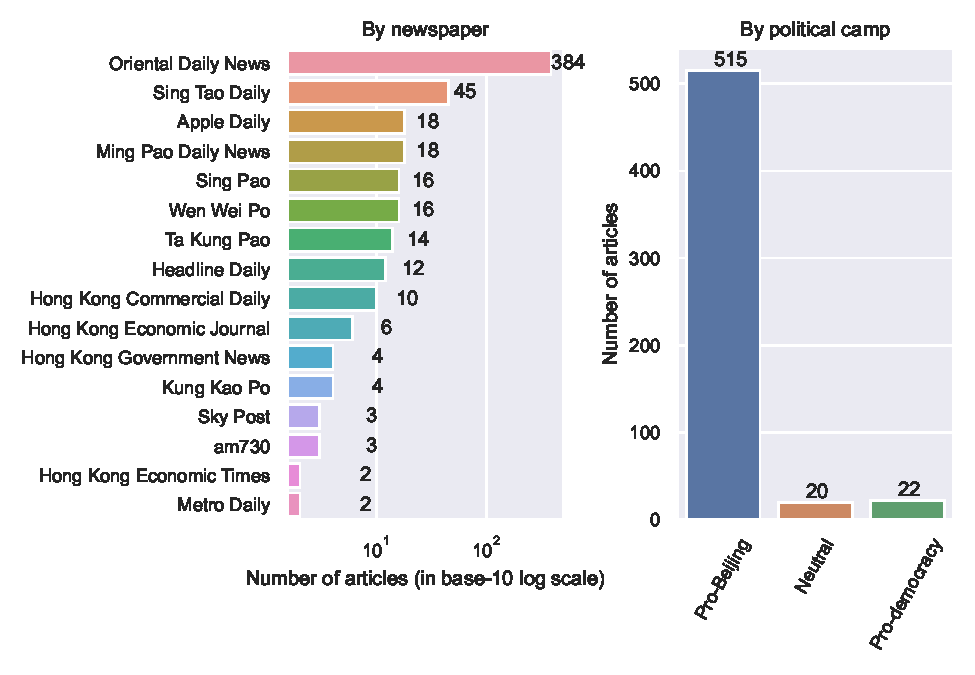
\includegraphics{versions/Chin_Chapter_4_2022-01-10_files/figure-latex/unnamed-chunk-1-1.pdf}
\caption{News articles on asylum seekers in 2019 by news outlet (left)
and political camp (right)}
\end{figure}

\begin{Shaded}
\begin{Highlighting}[]
\NormalTok{plt.clf()}
\end{Highlighting}
\end{Shaded}

Lastly, it will also be intriguing to see how the number of articles
might vary by month in 2019. As noted before, the anti-extradition law
protest lasted mostly from June to November when numerous large-scale
clashes between protesters and the police occurred. From figure 4.2, it
appears that coincidentally, there were the fewest amounts of articles
about asylum seekers published between August and November when some of
the most intense clashes (notably the \emph{siege} of the Hong Kong
Polytechnic University in November 2019) took place. Although
investigating whether the number of news articles about asylum seekers
may be correlated with that about the anti-extradition law protest would
be out of the scope of this paper, this could be a research question to
be pursued in another occasion.

\begin{Shaded}
\begin{Highlighting}[]
\NormalTok{articles\_by\_month }\OperatorTok{=}\NormalTok{ news\_df.Month.value\_counts(sort}\OperatorTok{=}\VariableTok{False}\NormalTok{)}
\NormalTok{ax }\OperatorTok{=}\NormalTok{ sns.lineplot(x}\OperatorTok{=}\NormalTok{articles\_by\_month.index, y}\OperatorTok{=}\NormalTok{articles\_by\_month, color}\OperatorTok{=}\StringTok{\textquotesingle{}tab:orange\textquotesingle{}}\NormalTok{)}
\NormalTok{ax.}\BuiltInTok{set}\NormalTok{(xlabel}\OperatorTok{=}\StringTok{\textquotesingle{}Month\textquotesingle{}}\NormalTok{, ylabel}\OperatorTok{=}\StringTok{\textquotesingle{}Number of articles\textquotesingle{}}\NormalTok{, xticks}\OperatorTok{=}\NormalTok{np.arange(}\DecValTok{1}\NormalTok{,}\DecValTok{13}\NormalTok{))}
\NormalTok{plt.tight\_layout()}
\NormalTok{plt.show()}
\end{Highlighting}
\end{Shaded}

\begin{figure}
\centering
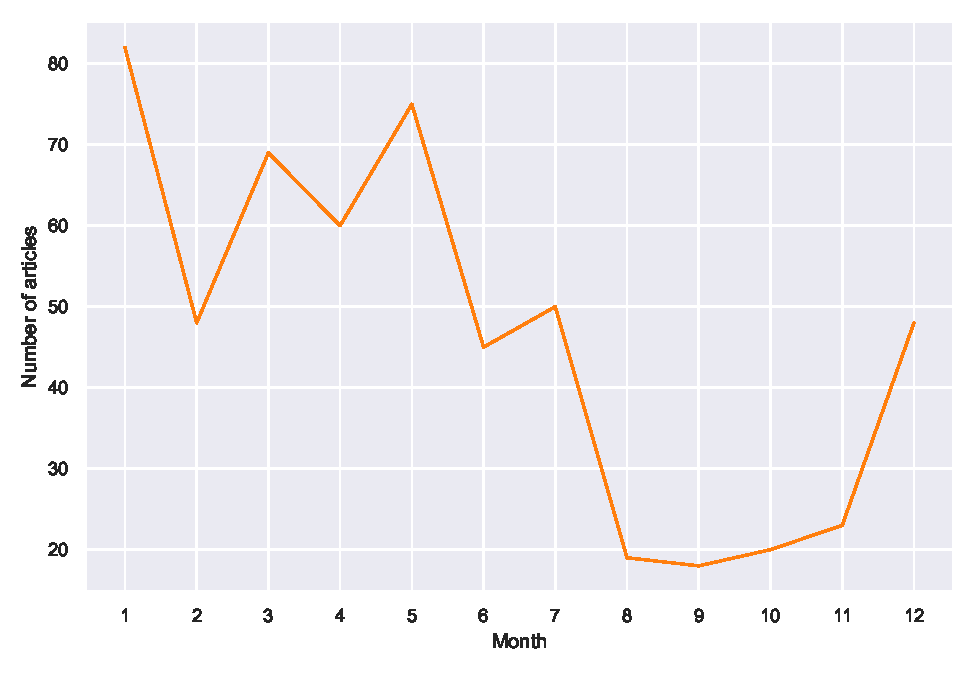
\includegraphics{versions/Chin_Chapter_4_2022-01-10_files/figure-latex/unnamed-chunk-2-3.pdf}
\caption{Temporal patterns of the publication of news articles about
asylum seekers in Hong Kong in 2019}
\end{figure}

\begin{Shaded}
\begin{Highlighting}[]
\NormalTok{plt.clf()}
\end{Highlighting}
\end{Shaded}

In short, the majority of news articles about non-refoulement claimants
in Hong Kong in 2019 were published by pro-Beijing media outlets, of
which a huge proportion was from Oriental Daily News. Moreover, the
number of articles by month was the lowest from August to November when
the anti-extradition law witnessed some of the most large-scale and
intense clashes.

\hypertarget{polarities-of-the-news-articles}{%
\subsection{Polarities of the news
articles}\label{polarities-of-the-news-articles}}

According to table 4.1, the polarity of the news articles about asylum
seekers in Hong Kong in 2019 tilted towards negative, since only around
4.3\% and 23.5\% of articles respectively depicted asylum seekers
positively and neutrally. The fact that the sentiment of the news
articles in 2019 was skewed towards negativity implies that I will need
to take class imbalance into account for modelling later.
Political-camp-wise, pro-Beijing media outlets had over 70\% of its
articles depicting asylum seekers in Hong Kong in negative lights,
whereas neutral and pro-democracy media outlets had their reportage
evenly spread between neutral and positive articles (albeit they
altogether constituted to only a small proportion of the total number of
articles in 2019). While H\textsubscript{1} shall be tested formally
with machine learning models after including other control variables
later, preliminary evidence suggests that the polarities of the news
articles vary with the political camp that the outlets belong to.

\begin{Shaded}
\begin{Highlighting}[]
\NormalTok{sentiment\_camp }\OperatorTok{=}\NormalTok{ pd.crosstab(news\_df.Political\_camp, news\_df.Sentiment, margins}\OperatorTok{=}\VariableTok{True}\NormalTok{)}
\NormalTok{sentiment\_camp.columns }\OperatorTok{=}\NormalTok{ [}\StringTok{"Negative"}\NormalTok{, }\StringTok{"Neutral"}\NormalTok{, }\StringTok{"Positive"}\NormalTok{, }\StringTok{"All"}\NormalTok{]}
\end{Highlighting}
\end{Shaded}

\begin{Shaded}
\begin{Highlighting}[]
\NormalTok{knitr}\SpecialCharTok{::}\FunctionTok{kable}\NormalTok{(py}\SpecialCharTok{$}\NormalTok{sentiment\_camp, }\AttributeTok{digits =} \DecValTok{4}\NormalTok{, }\AttributeTok{caption=}\StringTok{"Polarities of the news articles on asylum seekers in Hong Kong in 2019"}\NormalTok{)}
\end{Highlighting}
\end{Shaded}

\begin{longtable}[]{@{}lrrrr@{}}
\caption{Polarities of the news articles on asylum seekers in Hong Kong
in 2019}\tabularnewline
\toprule
& Negative & Neutral & Positive & All \\
\midrule
\endfirsthead
\toprule
& Negative & Neutral & Positive & All \\
\midrule
\endhead
Neutral & 0 & 12 & 8 & 20 \\
Pro-Beijing & 402 & 108 & 5 & 515 \\
Pro-democracy & 0 & 11 & 11 & 22 \\
All & 402 & 131 & 24 & 557 \\
\bottomrule
\end{longtable}

\hypertarget{presence-of-racial-labels}{%
\subsection{Presence of racial labels}\label{presence-of-racial-labels}}

Given the majority of asylum seekers in Hong Kong being non-ethnic
Chinese, it will also be worth glimpsing whether the presence of racial
labels for describing asylum seekers is associated with the sentiment of
the news articles. Judging from figure 4.3 preliminarily, however, it
appears that the patterns of the polarities are quite similar whether
news articles contain racial labels or not, namely, most of the articles
framed non-refoulement claimants negatively, and then some reported on
events about this group of population neutrally, and finally only a
small amount of articles were favourable towards asylum seekers residing
in the city. In any case, the machine learning model can add the
presence of racial labels as a control variable to test this potential
association more formally later.

\begin{Shaded}
\begin{Highlighting}[]
\NormalTok{ax }\OperatorTok{=}\NormalTok{ sns.countplot(x}\OperatorTok{=}\StringTok{"Racial\_label"}\NormalTok{, hue}\OperatorTok{=}\StringTok{"Sentiment"}\NormalTok{, data}\OperatorTok{=}\NormalTok{news\_df)}
\NormalTok{ax.}\BuiltInTok{set}\NormalTok{(xlabel}\OperatorTok{=}\StringTok{"Presence of racial labels"}\NormalTok{, ylabel}\OperatorTok{=}\StringTok{"Number of articles"}\NormalTok{)}
\NormalTok{ax.set\_xticklabels([}\StringTok{"No"}\NormalTok{, }\StringTok{"Yes"}\NormalTok{])}
\NormalTok{plt.show()}
\end{Highlighting}
\end{Shaded}

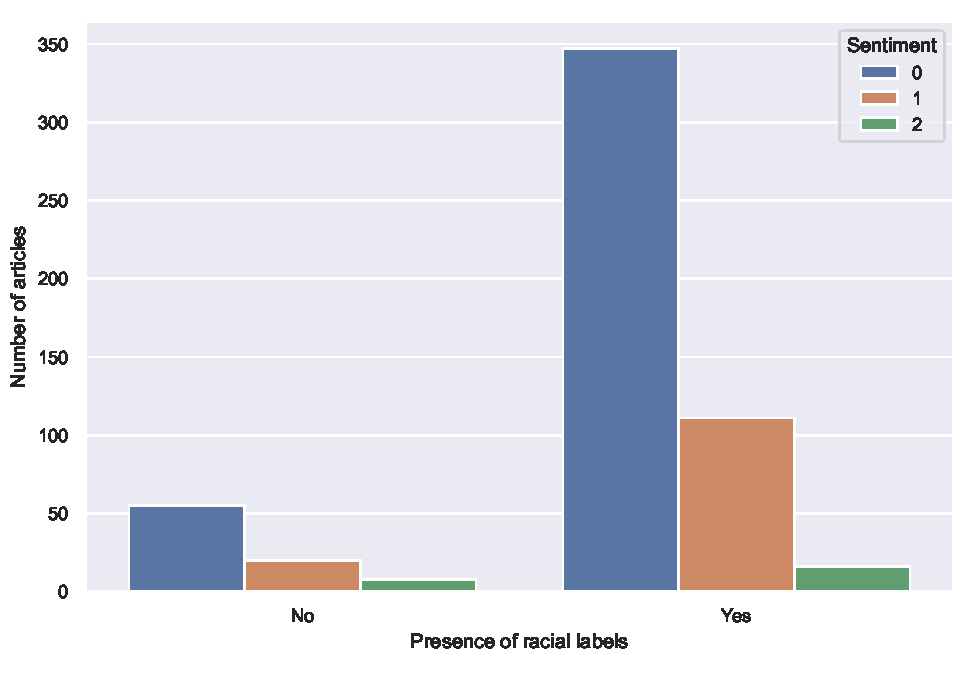
\includegraphics{versions/Chin_Chapter_4_2022-01-10_files/figure-latex/unnamed-chunk-5-1.pdf}

\begin{Shaded}
\begin{Highlighting}[]
\NormalTok{plt.clf()}
\end{Highlighting}
\end{Shaded}

\hypertarget{character-lengths-of-news-articles-and-titles}{%
\subsection{Character lengths of news articles and
titles}\label{character-lengths-of-news-articles-and-titles}}

Lastly, let's look at the distribution of the character lengths of the
titles and main texts of the news articles. According to figure 4.4 and
table 4.2, it appears that both the title and main text lengths have
right-skewed distributions. In other words, while most of the news
articles on asylum seekers in Hong Kong in 2019 had relatively short
titles and/or main texts, a few of them were considerably more verbose
than the rest of the articles.

\begin{Shaded}
\begin{Highlighting}[]
\NormalTok{fig, axes }\OperatorTok{=}\NormalTok{ plt.subplots(}\DecValTok{1}\NormalTok{, }\DecValTok{2}\NormalTok{)}

\CommentTok{\# Plotting distribution of title word count}
\NormalTok{sns.histplot(x}\OperatorTok{=}\StringTok{\textquotesingle{}Title\_length\textquotesingle{}}\NormalTok{, data}\OperatorTok{=}\NormalTok{news\_df, ax}\OperatorTok{=}\NormalTok{axes[}\DecValTok{0}\NormalTok{], color}\OperatorTok{=}\StringTok{\textquotesingle{}tab:blue\textquotesingle{}}\NormalTok{, alpha}\OperatorTok{=}\FloatTok{0.5}\NormalTok{)}
\NormalTok{axes[}\DecValTok{0}\NormalTok{].}\BuiltInTok{set}\NormalTok{(xlabel}\OperatorTok{=}\StringTok{\textquotesingle{}Word count\textquotesingle{}}\NormalTok{, title}\OperatorTok{=}\StringTok{\textquotesingle{}Article title\textquotesingle{}}\NormalTok{)}
\NormalTok{mean\_title\_length }\OperatorTok{=}\NormalTok{ news\_df.Title\_length.mean()}
\NormalTok{axes[}\DecValTok{0}\NormalTok{].axvline(mean\_title\_length, alpha}\OperatorTok{=}\FloatTok{0.5}\NormalTok{, linestyle }\OperatorTok{=} \StringTok{\textquotesingle{}{-}.\textquotesingle{}}\NormalTok{, c}\OperatorTok{=}\StringTok{\textquotesingle{}black\textquotesingle{}}\NormalTok{, label}\OperatorTok{=}\StringTok{\textquotesingle{}Mean of title length\textquotesingle{}}\NormalTok{)}
\NormalTok{axes[}\DecValTok{0}\NormalTok{].legend()}

\CommentTok{\# Plotting distribution of article word count}
\NormalTok{sns.histplot(x}\OperatorTok{=}\StringTok{\textquotesingle{}Raw\_article\_length\textquotesingle{}}\NormalTok{, data}\OperatorTok{=}\NormalTok{news\_df, ax}\OperatorTok{=}\NormalTok{axes[}\DecValTok{1}\NormalTok{], color}\OperatorTok{=}\StringTok{\textquotesingle{}tab:orange\textquotesingle{}}\NormalTok{, alpha}\OperatorTok{=}\FloatTok{0.5}\NormalTok{)}
\NormalTok{axes[}\DecValTok{1}\NormalTok{].}\BuiltInTok{set}\NormalTok{(xlabel}\OperatorTok{=}\StringTok{\textquotesingle{}Word count (in thousands)\textquotesingle{}}\NormalTok{, title}\OperatorTok{=}\StringTok{\textquotesingle{}Raw article text\textquotesingle{}}\NormalTok{)}
\NormalTok{mean\_article\_length }\OperatorTok{=}\NormalTok{ news\_df.Raw\_article\_length.mean()}
\NormalTok{axes[}\DecValTok{1}\NormalTok{].axvline(mean\_article\_length, alpha}\OperatorTok{=}\FloatTok{0.5}\NormalTok{, linestyle }\OperatorTok{=} \StringTok{\textquotesingle{}{-}{-}\textquotesingle{}}\NormalTok{, c}\OperatorTok{=}\StringTok{\textquotesingle{}black\textquotesingle{}}\NormalTok{, label}\OperatorTok{=}\StringTok{\textquotesingle{}Mean of main text length\textquotesingle{}}\NormalTok{)}
\NormalTok{axes[}\DecValTok{1}\NormalTok{].legend()}

\CommentTok{\# Global setup}
\NormalTok{plt.tight\_layout()}
\NormalTok{plt.show()}
\end{Highlighting}
\end{Shaded}

\begin{figure}
\centering
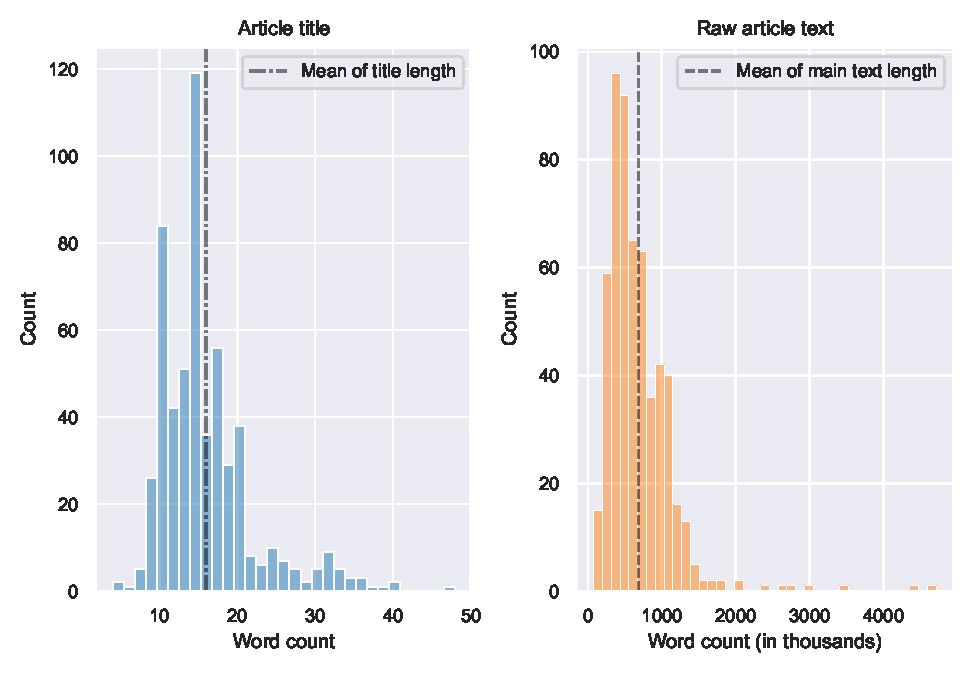
\includegraphics{versions/Chin_Chapter_4_2022-01-10_files/figure-latex/unnamed-chunk-6-3.pdf}
\caption{Distributions of the word counts of the articles' titles (left)
and main texts (right)}
\end{figure}

\begin{Shaded}
\begin{Highlighting}[]
\NormalTok{plt.clf()}
\end{Highlighting}
\end{Shaded}

\begin{Shaded}
\begin{Highlighting}[]
\NormalTok{article\_length\_summary }\OperatorTok{=}\NormalTok{ news\_df[[}\StringTok{\textquotesingle{}Title\_length\textquotesingle{}}\NormalTok{, }\StringTok{\textquotesingle{}Raw\_article\_length\textquotesingle{}}\NormalTok{]].describe()}
\end{Highlighting}
\end{Shaded}

\begin{Shaded}
\begin{Highlighting}[]
\NormalTok{knitr}\SpecialCharTok{::}\FunctionTok{kable}\NormalTok{(py}\SpecialCharTok{$}\NormalTok{article\_length\_summary, }\AttributeTok{col.names =} \FunctionTok{c}\NormalTok{(}\StringTok{"Title"}\NormalTok{, }\StringTok{"Raw main text"}\NormalTok{), }\AttributeTok{caption=}\StringTok{"Summary statistics of the word counts of the news articles\textquotesingle{} titles and main texts"}\NormalTok{)}
\end{Highlighting}
\end{Shaded}

\begin{longtable}[]{@{}lrr@{}}
\caption{Summary statistics of the word counts of the news articles'
titles and main texts}\tabularnewline
\toprule
& Title & Raw main text \\
\midrule
\endfirsthead
\toprule
& Title & Raw main text \\
\midrule
\endhead
count & 557.000000 & 557.0000 \\
mean & 15.965889 & 683.9264 \\
std & 5.993154 & 453.9607 \\
min & 4.000000 & 80.0000 \\
25\% & 12.000000 & 404.0000 \\
50\% & 15.000000 & 581.0000 \\
75\% & 18.000000 & 893.0000 \\
max & 48.000000 & 4715.0000 \\
\bottomrule
\end{longtable}

\hypertarget{sentiment-analysis}{%
\section{Sentiment analysis}\label{sentiment-analysis}}

\hypertarget{preprocessing}{%
\subsection{Preprocessing}\label{preprocessing}}

After making sense of the dataset with EDA, it is time to build the
sentiment analysis model to see whether the political affiliation of
news media outlets is associated with the polarities of the news
articles after controlling for other variables. But first there are some
preprocessing steps to be done so that the data are transformed into
suitable formats as inputs for machine learning models. For starters,
columns of the metadata should be excluded for being the inputs of the
models. Note that I have also removed the \texttt{Newspaper} column
since H\textsubscript{1} is more interested in whether newspaper outlets
of the pro-Beijing camp \emph{as a whole} may hold more negative
attitudes towards asylum seekers in Hong Kong vis-a-vis media outlets
with other political stances. The removed metadata columns are:
\texttt{Index,\ Date,\ Category,\ Page\_number} and \texttt{Newspaper}.

\begin{Shaded}
\begin{Highlighting}[]
\NormalTok{metadata\_columns }\OperatorTok{=}\NormalTok{ [}\StringTok{"Index"}\NormalTok{, }\StringTok{"Date"}\NormalTok{, }\StringTok{"Category"}\NormalTok{, }\StringTok{"Page\_number"}\NormalTok{, }\StringTok{"Newspaper"}\NormalTok{]}
\NormalTok{news\_df.drop(columns}\OperatorTok{=}\NormalTok{metadata\_columns, inplace}\OperatorTok{=}\VariableTok{True}\NormalTok{)}
\end{Highlighting}
\end{Shaded}

Furthermore, I have binned \texttt{Month} into four even split yearly
quarters (\texttt{Quarter}) to reduce the dimensionality of the dataset.
A further note on the categorical features is that they will need to be
transformed via one-hot encoding, meaning that each of them will be
transformed into \texttt{n} variables, with \texttt{n} being the number
of the original distinct values. Meanwhile, it would also be better to
standardise the numerical features (i.e.~other than
\texttt{Political\_camp} and \texttt{Quarter}) by centering theirs means
at 0 for better model convergence, but the standardiser should only be
fitted on the training set after splitting the data into the training
and validation sets in order to avoid data leakage (the same is also
true for creating the TF-IDF matrix). In any case, \texttt{sklearn}'s
\texttt{Pipeline} class allows me to perform both standardisation and
one-hot encoding conveniently later on.

\begin{Shaded}
\begin{Highlighting}[]
\CommentTok{\# Making pro{-}Beijing become the reference category}
\NormalTok{news\_df[}\StringTok{"Political\_camp"}\NormalTok{] }\OperatorTok{=}\NormalTok{ pd.Categorical(news\_df[}\StringTok{"Political\_camp"}\NormalTok{], categories}\OperatorTok{=}\NormalTok{[}\StringTok{\textquotesingle{}Pro{-}Beijing\textquotesingle{}}\NormalTok{, }\StringTok{\textquotesingle{}Neutral\textquotesingle{}}\NormalTok{, }\StringTok{\textquotesingle{}Pro{-}democracy\textquotesingle{}}\NormalTok{])  }

\CommentTok{\# Binning the months into four quarters}
\KeywordTok{def}\NormalTok{ quarter(x):}
  \ControlFlowTok{if}\NormalTok{ x }\OperatorTok{\textless{}=} \DecValTok{3}\NormalTok{:}
    \ControlFlowTok{return} \StringTok{"Q1"}
  \ControlFlowTok{elif}\NormalTok{ x }\OperatorTok{\textless{}=} \DecValTok{6}\NormalTok{:}
    \ControlFlowTok{return} \StringTok{"Q2"}
  \ControlFlowTok{elif}\NormalTok{ x }\OperatorTok{\textless{}=} \DecValTok{9}\NormalTok{:}
    \ControlFlowTok{return} \StringTok{"Q3"}
  \ControlFlowTok{else}\NormalTok{:}
    \ControlFlowTok{return} \StringTok{"Q4"}
\NormalTok{news\_df[}\StringTok{"Quarter"}\NormalTok{] }\OperatorTok{=}\NormalTok{ pd.Categorical(news\_df.Month.}\BuiltInTok{apply}\NormalTok{(quarter))}
\NormalTok{news\_df.drop(columns}\OperatorTok{=}\StringTok{"Month"}\NormalTok{, inplace}\OperatorTok{=}\VariableTok{True}\NormalTok{)}

\CommentTok{\# One{-}hot encoding}
\NormalTok{news\_df }\OperatorTok{=}\NormalTok{ pd.get\_dummies(news\_df, columns}\OperatorTok{=}\NormalTok{[}\StringTok{"Political\_camp"}\NormalTok{, }\StringTok{"Quarter"}\NormalTok{])}
\end{Highlighting}
\end{Shaded}

\begin{Shaded}
\begin{Highlighting}[]
\ImportTok{from}\NormalTok{ sklearn.model\_selection }\ImportTok{import}\NormalTok{ train\_test\_split}
\NormalTok{X }\OperatorTok{=}\NormalTok{ news\_df.drop(columns}\OperatorTok{=}\StringTok{"Sentiment"}\NormalTok{)}
\NormalTok{y }\OperatorTok{=}\NormalTok{ news\_df.Sentiment}
\NormalTok{X\_train, X\_test, y\_train, y\_test }\OperatorTok{=}\NormalTok{ train\_test\_split(X, y, test\_size}\OperatorTok{=}\FloatTok{0.2}\NormalTok{, stratify}\OperatorTok{=}\NormalTok{y, random\_state}\OperatorTok{=}\DecValTok{1}\NormalTok{)}
\end{Highlighting}
\end{Shaded}

The next step is to transform both the titles and main texts of the
articles into a TF-IDF term-document matrix. Apart from joining the
\texttt{Title} and \texttt{Text} columns together as the complete
\texttt{Article}, I will also add additional words into the dictionary
and remove stop words as well as punctuation for better tokenisation so
that the \texttt{NMF} model can better discover the latent topics.

\begin{Shaded}
\begin{Highlighting}[]
\CommentTok{\# Train set}
\NormalTok{X\_train[}\StringTok{"Article"}\NormalTok{] }\OperatorTok{=}\NormalTok{ X\_train.Title.}\BuiltInTok{str}\NormalTok{.cat(news\_df.Text, sep}\OperatorTok{=}\StringTok{" "}\NormalTok{)}
\NormalTok{X\_train.drop(columns}\OperatorTok{=}\NormalTok{[}\StringTok{"Text"}\NormalTok{, }\StringTok{"Title"}\NormalTok{], inplace}\OperatorTok{=}\VariableTok{True}\NormalTok{)}

\CommentTok{\# Test set}
\NormalTok{X\_test[}\StringTok{"Article"}\NormalTok{] }\OperatorTok{=}\NormalTok{ X\_test.Title.}\BuiltInTok{str}\NormalTok{.cat(news\_df.Text, sep}\OperatorTok{=}\StringTok{" "}\NormalTok{)}
\NormalTok{X\_test.drop(columns}\OperatorTok{=}\NormalTok{[}\StringTok{"Text"}\NormalTok{, }\StringTok{"Title"}\NormalTok{], inplace}\OperatorTok{=}\VariableTok{True}\NormalTok{)}
\end{Highlighting}
\end{Shaded}

\begin{Shaded}
\begin{Highlighting}[]
\KeywordTok{def}\NormalTok{ read\_text(path):}
    \ControlFlowTok{with} \BuiltInTok{open}\NormalTok{(path, }\StringTok{\textquotesingle{}r\textquotesingle{}}\NormalTok{, encoding}\OperatorTok{=}\StringTok{\textquotesingle{}utf{-}8\textquotesingle{}}\NormalTok{) }\ImportTok{as} \BuiltInTok{file}\NormalTok{:}
\NormalTok{        text }\OperatorTok{=} \BuiltInTok{file}\NormalTok{.readlines()}
\NormalTok{        text }\OperatorTok{=}\NormalTok{ [word.replace(}\StringTok{\textquotesingle{}}\CharTok{\textbackslash{}n}\StringTok{\textquotesingle{}}\NormalTok{, }\StringTok{\textquotesingle{}\textquotesingle{}}\NormalTok{) }\ControlFlowTok{for}\NormalTok{ word }\KeywordTok{in}\NormalTok{ text]}
        \ControlFlowTok{return}\NormalTok{ text}
\end{Highlighting}
\end{Shaded}

\begin{Shaded}
\begin{Highlighting}[]
\NormalTok{stop\_words\_cantonese }\OperatorTok{=}\NormalTok{ read\_text(}\StringTok{\textquotesingle{}Coding/text\_cleaning/cantonese\_stopwords.txt\textquotesingle{}}\NormalTok{)}
\NormalTok{punctuations }\OperatorTok{=}\NormalTok{ [punc }\ControlFlowTok{for}\NormalTok{ punc }\KeywordTok{in}\NormalTok{ zhon.hanzi.punctuation]}
\NormalTok{stop\_words\_full }\OperatorTok{=} \BuiltInTok{list}\NormalTok{(}\BuiltInTok{set}\NormalTok{(word }\ControlFlowTok{for}\NormalTok{ word }\KeywordTok{in}\NormalTok{ chain(stop\_words\_cantonese, punctuations)))  }
\end{Highlighting}
\end{Shaded}

To avoid data leakage as mentioned before, I will only fit the
\texttt{TfidfVectorizer} and the \texttt{NMF} models on the train set
(i.e.~\texttt{X\_train}) and then use the fitted instances to transform
both the train and test sets. Note that \texttt{NMF} is used here to
reduce the dimensionality of the dataset to prevent overfitting because
a typical TF-IDF matrix usually has thousands of columns (i.e.~tokens)
as features which will very likely cause the models to overfit on the
current dataset with only around 550 observations in total if the
term-document matrix is directly used as inputs. According to Stevens et
al. (\protect\hyperlink{ref-stevensExploringTopicCoherence2012}{2012})
(p.953), the matrix denoted as \emph{H} which captures the weight of
each topic (as columns) in each document (as rows) of the corpus can
help summarise the information of the articles in terms of which
topic(s) they primarily focus on.

I set the number of latent topics (\texttt{n\_components}) as 10 for the
\texttt{NMF} model, and this is decided based on figure 4.5 which plots
the reconstruction error measuring the difference of the values between
the original TF-IDF matrix and the reconstructed version after NMF.
Although there are certainly other valid choices of the number of latent
topics to be discovered by NMF, \texttt{10} appears to be a reasonable
choice as a compromise between finding out a wide variety of topics in
the corpus and not fitting too much into the noise of the data.

\begin{Shaded}
\begin{Highlighting}[]
\CommentTok{\# tokenizer}
\KeywordTok{def}\NormalTok{ tokenize\_zh(doc):}
  \ControlFlowTok{return}\NormalTok{ jieba.cut(doc)}

\CommentTok{\# Preprocessor}
\KeywordTok{def}\NormalTok{ preprocessor\_zh(doc):}
\NormalTok{  regex\_punctuation }\OperatorTok{=} \VerbatimStringTok{r"[\textbackslash{}d+\textbackslash{}s+\textbackslash{}n\textbackslash{}t]|[\textbackslash{}s+\textbackslash{}.\textbackslash{}!\textbackslash{}/\_,$\%\^{}*(+\textbackslash{}"\textbackslash{}\textquotesingle{}]+|[+——!,。?、\textasciitilde{}@\#¥\%……\&*()]+|[【】╮╯▽╰╭★→「」]+|[!,❤。~《》:()【】「」?”“;:、]"}
  \ControlFlowTok{return}\NormalTok{ re.sub(regex\_punctuation, }\StringTok{""}\NormalTok{, doc)}
\end{Highlighting}
\end{Shaded}

\begin{Shaded}
\begin{Highlighting}[]
\ImportTok{from}\NormalTok{ sklearn.feature\_extraction.text }\ImportTok{import}\NormalTok{ TfidfVectorizer}
\ImportTok{from}\NormalTok{ sklearn.decomposition }\ImportTok{import}\NormalTok{ NMF}

\CommentTok{\# Creating the tfidf matrix from the training set}
\NormalTok{tfidf\_vec }\OperatorTok{=}\NormalTok{ TfidfVectorizer(min\_df }\OperatorTok{=} \FloatTok{0.02}\NormalTok{,  }\CommentTok{\# Each token must appear in at least 2\% of the documents}
\NormalTok{                            preprocessor}\OperatorTok{=}\NormalTok{preprocessor\_zh, }
\NormalTok{                            tokenizer}\OperatorTok{=}\NormalTok{tokenize\_zh, }
\NormalTok{                            stop\_words}\OperatorTok{=}\NormalTok{stop\_words\_full)}
\NormalTok{X\_train\_tfidf }\OperatorTok{=}\NormalTok{ tfidf\_vec.fit\_transform(X\_train.Article)}

\CommentTok{\# Plotting the reconstruction error according to the number of latent topics}
\end{Highlighting}
\end{Shaded}

\begin{verbatim}
## C:\Users\kenji\ANACON~1\envs\py_397\lib\site-packages\sklearn\feature_extraction\text.py:396: UserWarning: Your stop_words may be inconsistent with your preprocessing. Tokenizing the stop words generated tokens ['介', '住', '便', '儻', '具體', '兼', '出', '前', '反過', '唷', '啪', '啷', '喔', '噠', '基', '天', '奈何', '始', '度', '庶', '怕', '成', '所述', '換句', '換言', '日', '梗', '樣', '死', '沒', '消', '然', '然之', '特', '甚', '相對', '真', '竟', '簡言', '綜上', '緊接', '總', '自個', '莫', '處', '見', '設', '說', '豈', '賊', '辦', '達', '鑒', '限', '難道', '雲', '非', '點兒'] not in stop_words.
##   warnings.warn(
\end{verbatim}

\begin{Shaded}
\begin{Highlighting}[]
\NormalTok{reconstruct\_error }\OperatorTok{=}\NormalTok{ []}
\ControlFlowTok{for}\NormalTok{ i }\KeywordTok{in} \BuiltInTok{range}\NormalTok{(}\DecValTok{1}\NormalTok{, }\DecValTok{21}\NormalTok{):}
\NormalTok{  nmf }\OperatorTok{=}\NormalTok{ NMF(n\_components}\OperatorTok{=}\NormalTok{i, max\_iter}\OperatorTok{=}\DecValTok{500}\NormalTok{, random\_state}\OperatorTok{=}\DecValTok{1}\NormalTok{)}
\NormalTok{  articles\_nmf }\OperatorTok{=}\NormalTok{ nmf.fit(X\_train\_tfidf)}
\NormalTok{  reconstruct\_error.append(nmf.reconstruction\_err\_)}

\NormalTok{ax }\OperatorTok{=}\NormalTok{ sns.lineplot(x}\OperatorTok{=}\NormalTok{np.arange(}\DecValTok{1}\NormalTok{, }\DecValTok{21}\NormalTok{), y}\OperatorTok{=}\NormalTok{reconstruct\_error)}
\NormalTok{ax.}\BuiltInTok{set}\NormalTok{(xlabel}\OperatorTok{=}\StringTok{"Number of latent topics"}\NormalTok{, ylabel}\OperatorTok{=}\StringTok{"Reconstruction error"}\NormalTok{, xticks}\OperatorTok{=}\NormalTok{np.arange(}\DecValTok{1}\NormalTok{, }\DecValTok{21}\NormalTok{))}
\NormalTok{plt.show()}
\end{Highlighting}
\end{Shaded}

\begin{figure}
\centering
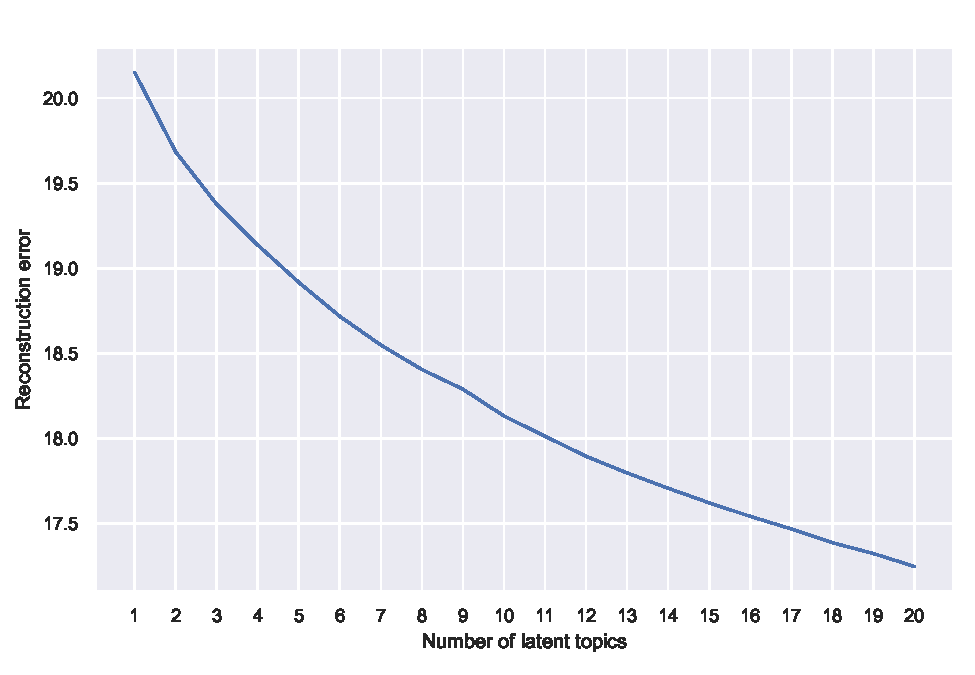
\includegraphics{versions/Chin_Chapter_4_2022-01-10_files/figure-latex/unnamed-chunk-9-1.pdf}
\caption{Elbow plot of the reconstruction error of NMF as a function of
the number of pre-specified latent topics}
\end{figure}

\begin{Shaded}
\begin{Highlighting}[]
\NormalTok{plt.clf()}

\CommentTok{\# Let\textquotesingle{}s set n\_components as 10 for nmf}
\NormalTok{nmf\_10 }\OperatorTok{=}\NormalTok{ NMF(n\_components}\OperatorTok{=}\DecValTok{10}\NormalTok{, max\_iter}\OperatorTok{=}\DecValTok{500}\NormalTok{, random\_state}\OperatorTok{=}\DecValTok{1}\NormalTok{)}
\NormalTok{X\_train\_nmf }\OperatorTok{=}\NormalTok{ nmf\_10.fit\_transform(X\_train\_tfidf)}
\end{Highlighting}
\end{Shaded}

In order to make the latent topics generated by the NMF model be named
more intuitive, I will inspect the 30 most prominent words of each
latent topic and then summarise each topic in a few words\footnote{A
  list of the 30 most prominent words in each of the topic and the code
  to generate it are available in the appendix.}. Overall, the ten
topics generated by NMF are more or less semantically coherent and can
be summed up concisely. Finally, I will transform the validation set's
articles with the fitted instance of the TF-IDF and NMF models with the
training set.

\begin{Shaded}
\begin{Highlighting}[]
\CommentTok{\# Naming the latent topics more precisely}
\NormalTok{topics\_list }\OperatorTok{=}\NormalTok{ [}\StringTok{"Crimes"}\NormalTok{, }\StringTok{"Non{-}refoulement policy"}\NormalTok{, }\StringTok{"Illegal labours"}\NormalTok{, }\StringTok{"Illegal gambling"}\NormalTok{, }\StringTok{"Drugs"}\NormalTok{, }\StringTok{"Illegal immigration"}\NormalTok{, }\StringTok{"Murder"}\NormalTok{, }\StringTok{"Robbery"}\NormalTok{, }\StringTok{"South Asian settlements"}\NormalTok{, }\StringTok{"Public security"}\NormalTok{]}

\CommentTok{\# Concatenating the NMF DataFrame for the training set}
\NormalTok{X\_train\_nmf\_df }\OperatorTok{=}\NormalTok{ pd.DataFrame(X\_train\_nmf, index}\OperatorTok{=}\NormalTok{X\_train.index, columns}\OperatorTok{=}\NormalTok{topics\_list)}
\NormalTok{X\_train\_final }\OperatorTok{=}\NormalTok{ pd.concat([X\_train, X\_train\_nmf\_df], axis}\OperatorTok{=}\DecValTok{1}\NormalTok{)}
\NormalTok{X\_train\_final.drop(columns}\OperatorTok{=}\StringTok{"Article"}\NormalTok{, inplace}\OperatorTok{=}\VariableTok{True}\NormalTok{)}

\CommentTok{\# Concatenating the NMF DataFrame for the validation set}
\NormalTok{X\_test\_tfidf }\OperatorTok{=}\NormalTok{ tfidf\_vec.transform(X\_test.Article)}
\NormalTok{X\_test\_nmf }\OperatorTok{=}\NormalTok{ nmf\_10.transform(X\_test\_tfidf)}
\NormalTok{X\_test\_nmf\_df }\OperatorTok{=}\NormalTok{ pd.DataFrame(X\_test\_nmf, index}\OperatorTok{=}\NormalTok{X\_test.index, columns}\OperatorTok{=}\NormalTok{topics\_list)}
\NormalTok{X\_test\_final }\OperatorTok{=}\NormalTok{ pd.concat([X\_test, X\_test\_nmf\_df], axis}\OperatorTok{=}\DecValTok{1}\NormalTok{)}
\NormalTok{X\_test\_final.drop(columns}\OperatorTok{=}\StringTok{"Article"}\NormalTok{, inplace}\OperatorTok{=}\VariableTok{True}\NormalTok{)}
\end{Highlighting}
\end{Shaded}

\hypertarget{training-the-model}{%
\subsection{Training the model}\label{training-the-model}}

After the above preprocessing steps, it is time to train a model that
adequately predicts the relations between the features and the sentiment
of the articles before finding out the importance of the political camp
as the main independent variable. To facilitate the decision of which
model to use and model tuning, I will first run some baseline models
with the default hyper-parameters, except that I have adjusted the
weights of each class in the dependent variable due to class imbalance
and also tweaked the \texttt{n\_estimators} of the XGBoost model to 15
instead of the default value of 200 to prevent the model from being too
big\footnote{For the complete documentation of the default parameters of
  the models used in this thesis, refer to the websites of
  \href{scikit-learn:\%20machine\%20learning\%20in\%20Python\%20—\%20scikit-learn\%201.0.2\%20documentation}{scikit-learn}
  and \href{https://xgboost.readthedocs.io/en/stable/}{XGBoost
  Documentation --- xgboost 1.5.1 documentation}.}. Moreover, tree-based
models (i.e.~random forest and xgboost) do not necessarily need to have
the numerical features standardised, and thus only the categorical
columns need to be one-hot encoded. The baseline models will be compared
based on their performance on log loss in 5-fold cross validation and on
the testing set.

\begin{Shaded}
\begin{Highlighting}[]
\ImportTok{from}\NormalTok{ sklearn.model\_selection }\ImportTok{import}\NormalTok{ cross\_val\_score, StratifiedKFold}
\ImportTok{from}\NormalTok{ sklearn.metrics }\ImportTok{import}\NormalTok{ log\_loss}

\CommentTok{\# Defining the kfold strategy}
\NormalTok{five\_fold\_cv }\OperatorTok{=}\NormalTok{ StratifiedKFold(n\_splits}\OperatorTok{=}\DecValTok{5}\NormalTok{, shuffle}\OperatorTok{=}\VariableTok{True}\NormalTok{, random\_state}\OperatorTok{=}\DecValTok{1}\NormalTok{)}

\CommentTok{\# Utility function for evaluating the model\textquotesingle{}s performance in cross validation and test set in terms of log loss}
\KeywordTok{def}\NormalTok{ evaluate\_model(model, model\_name: }\BuiltInTok{str}\NormalTok{, cv}\OperatorTok{=}\NormalTok{five\_fold\_cv, X\_train}\OperatorTok{=}\NormalTok{X\_train\_final, X\_test}\OperatorTok{=}\NormalTok{X\_test\_final, y\_train}\OperatorTok{=}\NormalTok{y\_train, y\_test}\OperatorTok{=}\NormalTok{y\_test):}
\NormalTok{  cv\_log\_loss }\OperatorTok{=}\NormalTok{ np.mean(}\OperatorTok{{-}}\NormalTok{cross\_val\_score(model, X\_train, y\_train, cv}\OperatorTok{=}\NormalTok{cv, scoring}\OperatorTok{=}\StringTok{"neg\_log\_loss"}\NormalTok{))}
\NormalTok{  y\_pred\_proba }\OperatorTok{=}\NormalTok{ model.predict\_proba(X\_test)}
\NormalTok{  test\_log\_loss }\OperatorTok{=}\NormalTok{ log\_loss(y\_test, y\_pred\_proba)}
  \ControlFlowTok{return}\NormalTok{ \{}\StringTok{"5{-}fold cv log loss"}\NormalTok{: cv\_log\_loss, }\StringTok{"Test set log loss"}\NormalTok{: test\_log\_loss\}}
  
\end{Highlighting}
\end{Shaded}

\begin{Shaded}
\begin{Highlighting}[]
\ImportTok{from}\NormalTok{ sklearn.preprocessing }\ImportTok{import}\NormalTok{ StandardScaler, OneHotEncoder}
\ImportTok{from}\NormalTok{ sklearn.compose }\ImportTok{import}\NormalTok{ ColumnTransformer}

\CommentTok{\# Separating the columns for respective preprocessing steps}
\NormalTok{numeric\_columns }\OperatorTok{=}\NormalTok{ [col }\ControlFlowTok{for}\NormalTok{ col }\KeywordTok{in}\NormalTok{ X\_train\_final.columns }\ControlFlowTok{if}\NormalTok{ X\_train\_final[col].dtype }\KeywordTok{in}\NormalTok{ [}\StringTok{"int64"}\NormalTok{, }\StringTok{"float64"}\NormalTok{] }\KeywordTok{and}\NormalTok{ col }\OperatorTok{!=} \StringTok{"Racial\_label"}\NormalTok{]}

\CommentTok{\# Preprocessor for linear models}
\NormalTok{stand\_preprocessor }\OperatorTok{=}\NormalTok{ ColumnTransformer([(}\StringTok{"standardiser"}\NormalTok{, StandardScaler(), numeric\_columns)],}
\NormalTok{                                         remainder}\OperatorTok{=}\StringTok{\textquotesingle{}passthrough\textquotesingle{}}\NormalTok{)}
\NormalTok{\_ }\OperatorTok{=}\NormalTok{ stand\_preprocessor.fit(X\_train\_final)}
\end{Highlighting}
\end{Shaded}

\begin{Shaded}
\begin{Highlighting}[]
\ImportTok{from}\NormalTok{ sklearn.linear\_model }\ImportTok{import}\NormalTok{ LogisticRegression}
\ImportTok{from}\NormalTok{ sklearn.svm }\ImportTok{import}\NormalTok{ SVC}
\ImportTok{from}\NormalTok{ sklearn.ensemble }\ImportTok{import}\NormalTok{ RandomForestClassifier}
\ImportTok{from}\NormalTok{ sklearn.pipeline }\ImportTok{import}\NormalTok{ Pipeline}
\ImportTok{from}\NormalTok{ sklearn.utils.class\_weight }\ImportTok{import}\NormalTok{ compute\_sample\_weight}
\ImportTok{import}\NormalTok{ xgboost }\ImportTok{as}\NormalTok{ xgb}

\CommentTok{\# Logistic regression pipeline}
\NormalTok{log\_reg\_baseline }\OperatorTok{=}\NormalTok{ Pipeline([(}\StringTok{"preprocess"}\NormalTok{, stand\_preprocessor), }
\NormalTok{                             (}\StringTok{"log\_reg"}\NormalTok{, LogisticRegression(random\_state}\OperatorTok{=}\DecValTok{1}\NormalTok{,  }
\NormalTok{                                                            class\_weight}\OperatorTok{=}\StringTok{"balanced"}\NormalTok{))])}
\NormalTok{\_ }\OperatorTok{=}\NormalTok{ log\_reg\_baseline.fit(X\_train\_final, y\_train)}
\NormalTok{log\_reg\_base\_result }\OperatorTok{=}\NormalTok{ evaluate\_model(log\_reg\_baseline, }\StringTok{"baseline logistic regression"}\NormalTok{)}

\CommentTok{\# SVM pipeline}
\NormalTok{svm\_baseline }\OperatorTok{=}\NormalTok{ Pipeline([(}\StringTok{"preprocess"}\NormalTok{, stand\_preprocessor), }
\NormalTok{                         (}\StringTok{"svm"}\NormalTok{, SVC(probability}\OperatorTok{=}\VariableTok{True}\NormalTok{, class\_weight}\OperatorTok{=}\StringTok{"balanced"}\NormalTok{, random\_state}\OperatorTok{=}\DecValTok{1}\NormalTok{))])}
\NormalTok{\_ }\OperatorTok{=}\NormalTok{ svm\_baseline.fit(X\_train\_final, y\_train)}
\NormalTok{svm\_base\_result }\OperatorTok{=}\NormalTok{ evaluate\_model(svm\_baseline, }\StringTok{"baseline support vector machine"}\NormalTok{)}

\CommentTok{\# Random forest pipeline}
\NormalTok{rf\_baseline }\OperatorTok{=}\NormalTok{ RandomForestClassifier(class\_weight}\OperatorTok{=}\StringTok{"balanced"}\NormalTok{, random\_state}\OperatorTok{=}\DecValTok{1}\NormalTok{, criterion}\OperatorTok{=}\StringTok{"entropy"}\NormalTok{)}
\NormalTok{\_ }\OperatorTok{=}\NormalTok{ rf\_baseline.fit(X\_train\_final, y\_train)}
\NormalTok{rf\_base\_result }\OperatorTok{=}\NormalTok{ evaluate\_model(rf\_baseline, }\StringTok{"baseline random forest"}\NormalTok{)}

\CommentTok{\# xgboost pipeline}
\NormalTok{xgb\_sample\_weight }\OperatorTok{=}\NormalTok{ compute\_sample\_weight(class\_weight}\OperatorTok{=}\StringTok{"balanced"}\NormalTok{, y}\OperatorTok{=}\NormalTok{y\_train)}
\NormalTok{xgboost\_baseline }\OperatorTok{=}\NormalTok{ xgb.XGBClassifier(n\_estimators}\OperatorTok{=}\DecValTok{15}\NormalTok{,}
\NormalTok{                                     objective}\OperatorTok{=}\StringTok{"multi:softmax"}\NormalTok{,}
\NormalTok{                                     eval\_metric}\OperatorTok{=}\StringTok{"mlogloss"}\NormalTok{,}
\NormalTok{                                     random\_state}\OperatorTok{=}\DecValTok{1}\NormalTok{, }
\NormalTok{                                     use\_label\_encoder}\OperatorTok{=}\VariableTok{False}\NormalTok{)}
\NormalTok{\_ }\OperatorTok{=}\NormalTok{ xgboost\_baseline.fit(X\_train\_final, }
\NormalTok{                         y\_train, }
\NormalTok{                         sample\_weight}\OperatorTok{=}\NormalTok{xgb\_sample\_weight)}
\NormalTok{xgb\_base\_result }\OperatorTok{=}\NormalTok{ evaluate\_model(xgboost\_baseline, }\StringTok{"baseline XGBoost"}\NormalTok{)}

\CommentTok{\# Creating the DataFrame of the baseline results}
\NormalTok{baseline\_log\_loss\_df }\OperatorTok{=}\NormalTok{ pd.DataFrame([log\_reg\_base\_result, svm\_base\_result, rf\_base\_result, xgb\_base\_result], index}\OperatorTok{=}\NormalTok{[}\StringTok{"Logistic regression"}\NormalTok{, }\StringTok{"SVM"}\NormalTok{, }\StringTok{"Random forest"}\NormalTok{, }\StringTok{"XGBoost classifier"}\NormalTok{])}
\end{Highlighting}
\end{Shaded}

\begin{Shaded}
\begin{Highlighting}[]
\NormalTok{knitr}\SpecialCharTok{::}\FunctionTok{kable}\NormalTok{(py}\SpecialCharTok{$}\NormalTok{baseline\_log\_loss\_df, }\AttributeTok{caption =} \StringTok{"Log loss on 5{-}fold cv and test set for the 4 baseline models"}\NormalTok{)}
\end{Highlighting}
\end{Shaded}

\begin{longtable}[]{@{}lrr@{}}
\caption{Log loss on 5-fold cv and test set for the 4 baseline
models}\tabularnewline
\toprule
& 5-fold cv log loss & Test set log loss \\
\midrule
\endfirsthead
\toprule
& 5-fold cv log loss & Test set log loss \\
\midrule
\endhead
Logistic regression & 0.4648889 & 0.3495389 \\
SVM & 0.4416793 & 0.3371468 \\
Random forest & 0.3805292 & 0.3466180 \\
XGBoost classifier & 0.3863108 & 0.2859553 \\
\bottomrule
\end{longtable}

Table 4.3 contains the performance of the log loss on both the 5-fold
cross validation and test set log loss scores for the four baseline
models. Judging by the performance of log loss on the test set, it seems
that the XGBoost model performs the best out of all candidates. I will
then perform some hyperparameter tuning of the XGBoost model to see if
there could be any improvements of its performance\footnote{The code for
  tuning the model can be found in the appendix.}. Surprisingly, the
tuned XGBoost model has a higher log loss on the test data than the
pre-tuned one. If we look at the per-class f1 score in tables 4.4 and
4.5, however, we can see that the tuned XGBoost model performs
considerably better in the f1 score for predicting whether a news
article's polarity is positive or not (i.e., class \texttt{2}).
Therefore, I will use the tuned model as the basis of interpreting the
impact of the features on predicting the sentiments of the news articles
about asylum seekers in Hong Kong in 2019.

\begin{Shaded}
\begin{Highlighting}[]
\CommentTok{\# Loading the tuned model}
\ImportTok{import}\NormalTok{ pickle}
\NormalTok{xgboost\_tuned }\OperatorTok{=}\NormalTok{ pickle.load(}\BuiltInTok{open}\NormalTok{(}\StringTok{"xgb\_clf.pkl"}\NormalTok{, }\StringTok{"rb"}\NormalTok{))}

\CommentTok{\# Creating the DataFrames for f1 score of both baseline and tuned models}
\ImportTok{from}\NormalTok{ sklearn.metrics }\ImportTok{import}\NormalTok{ classification\_report}
\NormalTok{xgb\_base\_class\_report }\OperatorTok{=}\NormalTok{ pd.DataFrame(classification\_report(y\_test, xgboost\_baseline.predict(X\_test\_final), output\_dict}\OperatorTok{=}\VariableTok{True}\NormalTok{)).T}
\NormalTok{xgb\_tuned\_class\_report }\OperatorTok{=}\NormalTok{ pd.DataFrame(classification\_report(y\_test, xgboost\_tuned.predict(X\_test\_final), output\_dict}\OperatorTok{=}\VariableTok{True}\NormalTok{)).T}
\end{Highlighting}
\end{Shaded}

\begin{Shaded}
\begin{Highlighting}[]
\NormalTok{knitr}\SpecialCharTok{::}\FunctionTok{kable}\NormalTok{(py}\SpecialCharTok{$}\NormalTok{xgb\_base\_class\_report, }\AttributeTok{digits=}\DecValTok{4}\NormalTok{, }\AttributeTok{caption=}\StringTok{"Classification report of the baseline XGBoost model"}\NormalTok{)}
\end{Highlighting}
\end{Shaded}

\begin{longtable}[]{@{}lrrrr@{}}
\caption{Classification report of the baseline XGBoost
model}\tabularnewline
\toprule
& precision & recall & f1-score & support \\
\midrule
\endfirsthead
\toprule
& precision & recall & f1-score & support \\
\midrule
\endhead
0 & 0.8953 & 0.9506 & 0.9222 & 81.000 \\
1 & 0.7826 & 0.6923 & 0.7347 & 26.000 \\
2 & 1.0000 & 0.6000 & 0.7500 & 5.000 \\
accuracy & 0.8750 & 0.8750 & 0.8750 & 0.875 \\
macro avg & 0.8927 & 0.7476 & 0.8023 & 112.000 \\
weighted avg & 0.8738 & 0.8750 & 0.8710 & 112.000 \\
\bottomrule
\end{longtable}

\begin{Shaded}
\begin{Highlighting}[]
\NormalTok{knitr}\SpecialCharTok{::}\FunctionTok{kable}\NormalTok{(py}\SpecialCharTok{$}\NormalTok{xgb\_tuned\_class\_report, }\AttributeTok{digits=}\DecValTok{4}\NormalTok{, }\AttributeTok{caption=}\StringTok{"Classification report of the tuned XGBoost model"}\NormalTok{)}
\end{Highlighting}
\end{Shaded}

\begin{longtable}[]{@{}lrrrr@{}}
\caption{Classification report of the tuned XGBoost
model}\tabularnewline
\toprule
& precision & recall & f1-score & support \\
\midrule
\endfirsthead
\toprule
& precision & recall & f1-score & support \\
\midrule
\endhead
0 & 0.9259 & 0.9259 & 0.9259 & 81.0000 \\
1 & 0.7407 & 0.7692 & 0.7547 & 26.0000 \\
2 & 1.0000 & 0.8000 & 0.8889 & 5.0000 \\
accuracy & 0.8839 & 0.8839 & 0.8839 & 0.8839 \\
macro avg & 0.8889 & 0.8317 & 0.8565 & 112.0000 \\
weighted avg & 0.8862 & 0.8839 & 0.8845 & 112.0000 \\
\bottomrule
\end{longtable}

\hypertarget{is-the-pro-beijing-camp-more-likely-to-portray-asylum-seekers-in-2019-more-negatively-than-other-outlets}{%
\subsection{Is the pro-Beijing camp more likely to portray asylum
seekers in 2019 more negatively than other
outlets?}\label{is-the-pro-beijing-camp-more-likely-to-portray-asylum-seekers-in-2019-more-negatively-than-other-outlets}}

We can use SHAP values
(\protect\hyperlink{ref-lundbergSlundbergShap2022}{Lundberg 2022}) which
evaluates how much impact each feature has on the model prediction
between taking certain values and its baseline value. The higher the
SHAP values of a feature, the higher its impact of the model's
prediction. According to figure 4.6, we can see that on the level of the
whole XGBoost model, whether a media belongs to the pro-Beijing camp or
not (\texttt{Political\_camp\_Pro-Beijing}) is the fourth most important
features in predicting the sentiment of a news article, only being lower
than the magnitudes of three themes of the news articles about asylum
seekers (i.e., public security, murder and crimes). Specifically,
pro-Beijing affiliation has the second largest magnitude in affecting
the prediction of whether a news article has a negative narrative
against non-refoulement claimants, as one can see the pink bar
representing the impact of a feature on predicting class \texttt{0} in
the model is the second longest for the
\texttt{Political\_camp\_Pro-Beijing} feature (only behind that of the
theme \texttt{Crimes} in the articles). Let's zoom into the SHAP values
plot for predicting class \texttt{0}.

\begin{Shaded}
\begin{Highlighting}[]
\CommentTok{\# Setting up the shap values }
\ImportTok{import}\NormalTok{ shap}
\NormalTok{xgb\_explainer }\OperatorTok{=}\NormalTok{ shap.TreeExplainer(xgboost\_tuned)}
\NormalTok{xgb\_shap\_values }\OperatorTok{=}\NormalTok{ xgb\_explainer.shap\_values(X\_test\_final)}

\CommentTok{\# Defining the plotting function}
\end{Highlighting}
\end{Shaded}

\begin{verbatim}
## ntree_limit is deprecated, use `iteration_range` or model slicing instead.
\end{verbatim}

\begin{Shaded}
\begin{Highlighting}[]
\KeywordTok{def}\NormalTok{ plot\_shap\_values(class\_label}\OperatorTok{=}\VariableTok{None}\NormalTok{, }\OperatorTok{**}\NormalTok{kwargs):}
  \ControlFlowTok{if}\NormalTok{ class\_label }\OperatorTok{==} \VariableTok{None}\NormalTok{:}
\NormalTok{    shap.summary\_plot(xgb\_shap\_values, X\_test\_final, }\OperatorTok{**}\NormalTok{kwargs)}
\NormalTok{    plt.clf()}
  \ControlFlowTok{else}\NormalTok{:}
\NormalTok{    shap.summary\_plot(xgb\_shap\_values[class\_label], X\_test\_final, }\OperatorTok{**}\NormalTok{kwargs)}
\NormalTok{    plt.clf()}
    
\end{Highlighting}
\end{Shaded}

\begin{Shaded}
\begin{Highlighting}[]
\NormalTok{plot\_shap\_values()}
\end{Highlighting}
\end{Shaded}

\begin{figure}
\centering
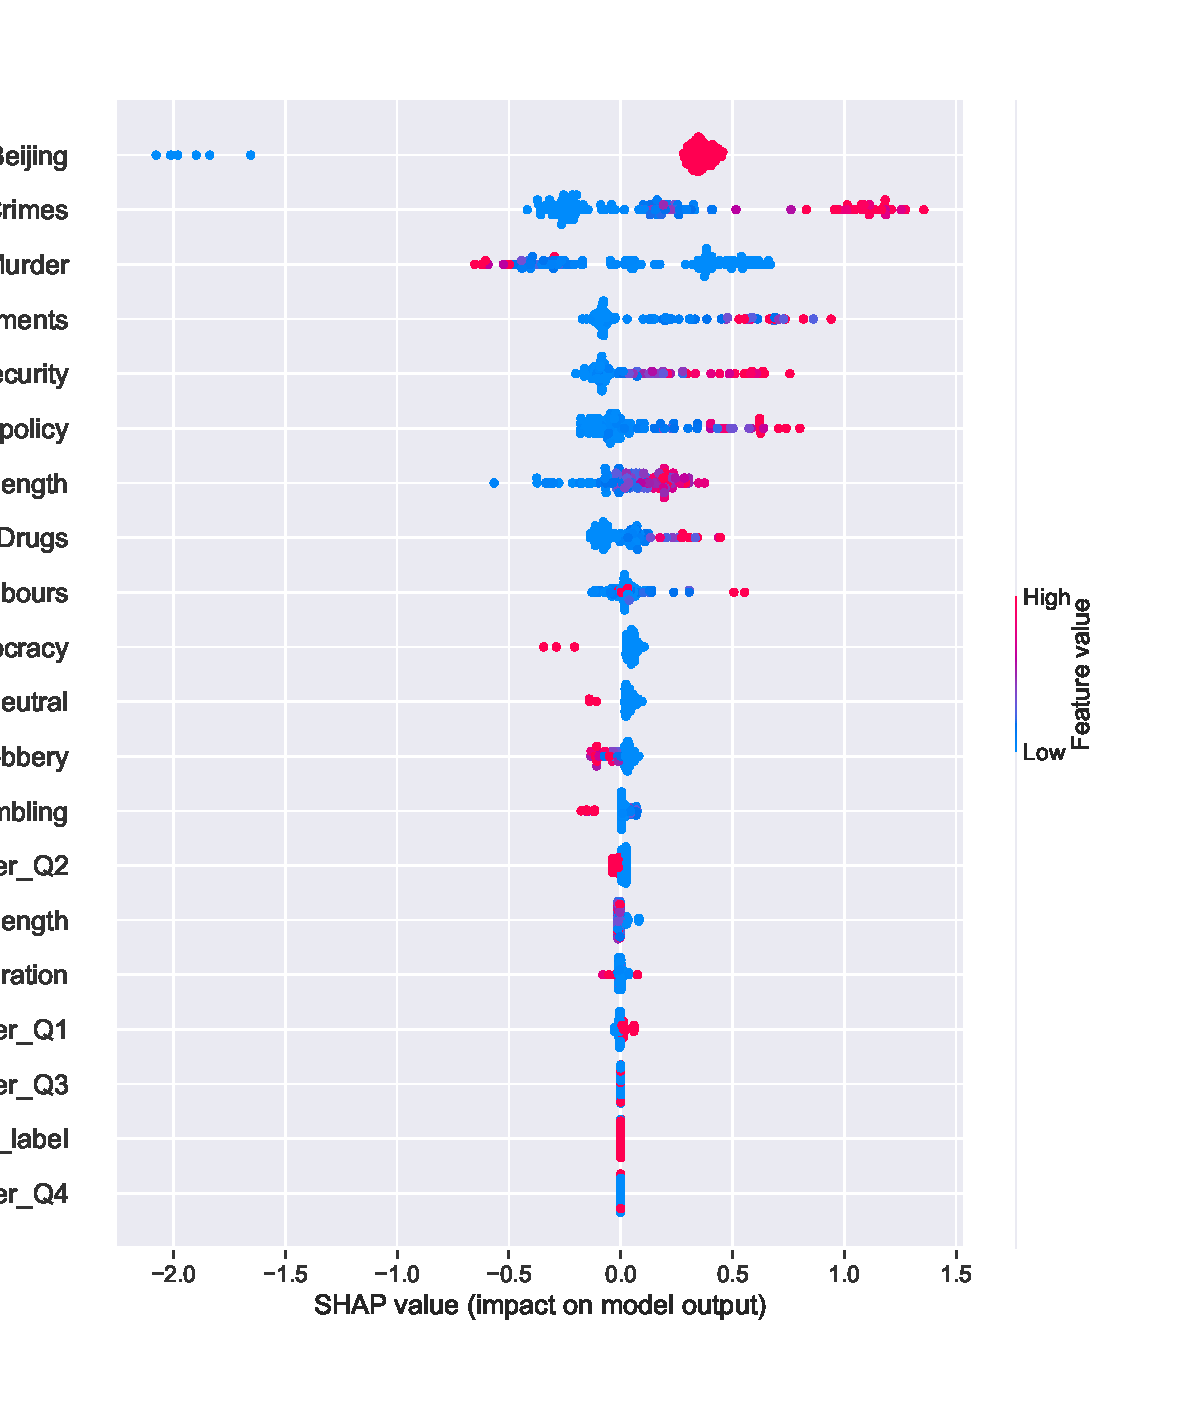
\includegraphics{versions/Chin_Chapter_4_2022-01-10_files/figure-latex/unnamed-chunk-13-1.pdf}
\caption{The overall SHAP values of the features in the model's
predictions and their impact by class}
\end{figure}

The beeswarm plot in figure 4.7 zooms into the importance of each
feature in predicting whether a news article on asylum seekers has a
negative (coded as \texttt{0}) polarity, and features appearing at the
top of the y-axis are deemed more important than those at the lower end
of the y-axis. In a SHAP value beeswarm plot, dots in red mean the value
of a feature is high (or present in case of a binary feature,
e.g.~one-hot-encoded columns), whereas those in blue mean the value of a
feature is low (or absent in the case of a binary feature). As one can
see, not only is the affiliation to pro-Beijing camp the second most
determinant feature in predicting whether a news article has negative
polarity, but such affiliation will also increase the probability of a
news articles portraying asylum seekers in negative lights.

\begin{Shaded}
\begin{Highlighting}[]
\NormalTok{plot\_shap\_values(}\DecValTok{0}\NormalTok{)}
\end{Highlighting}
\end{Shaded}

\begin{figure}
\centering
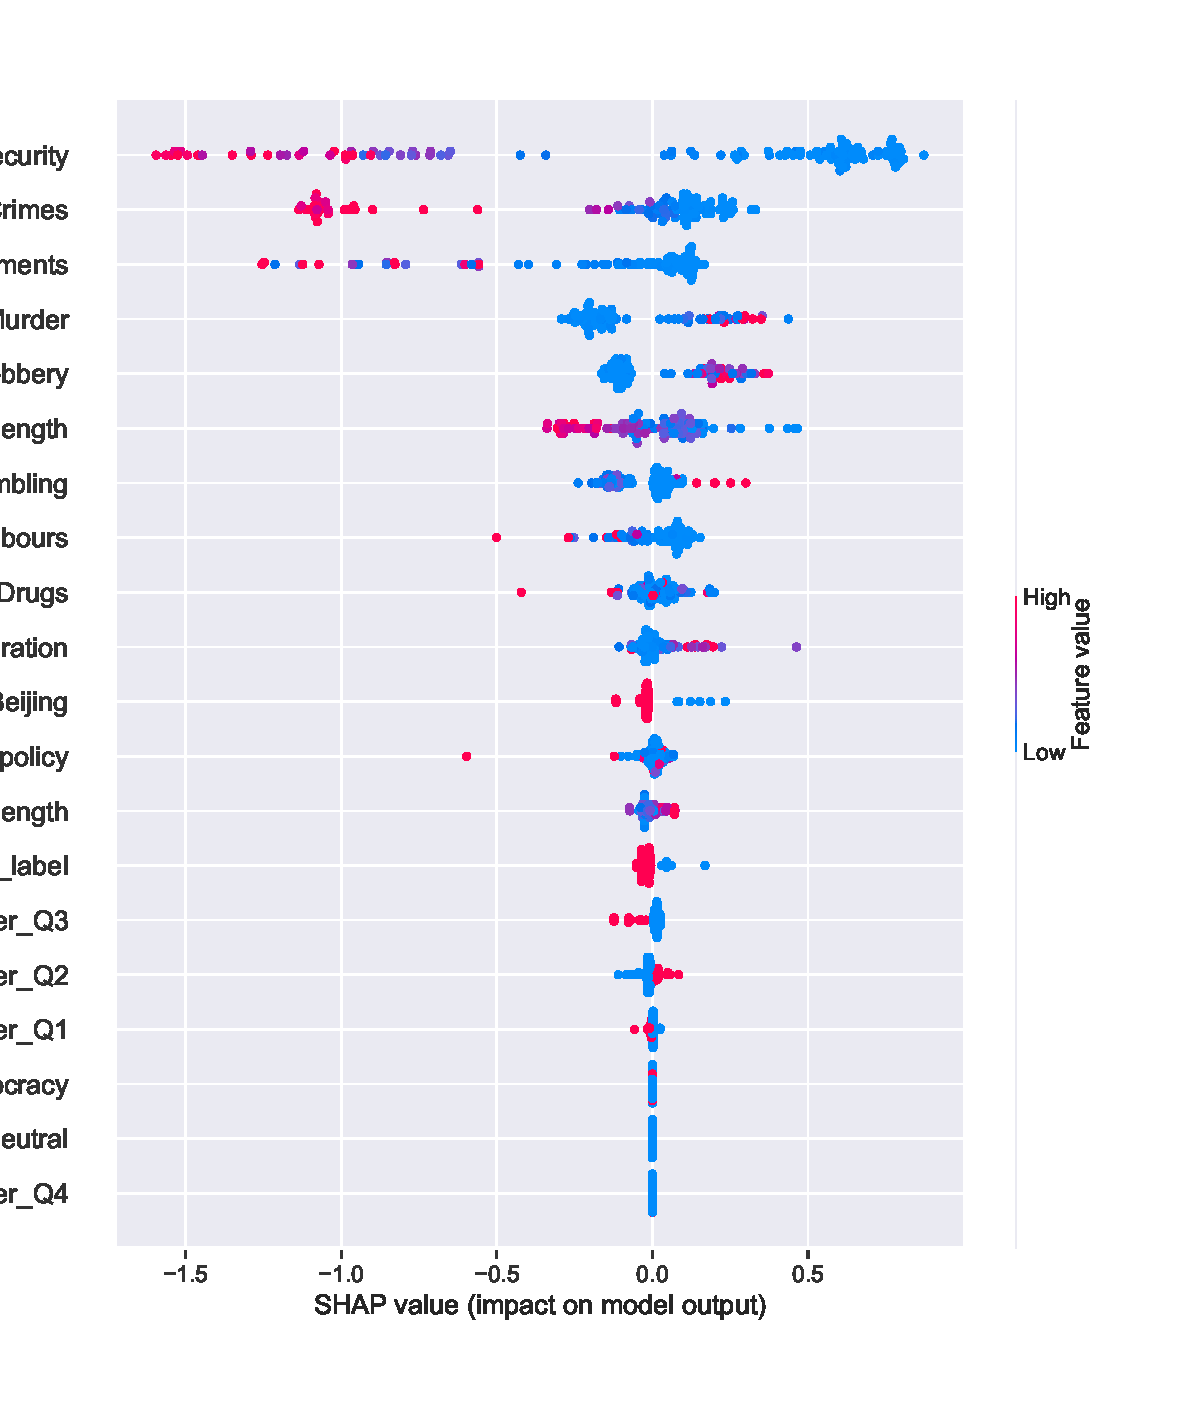
\includegraphics{versions/Chin_Chapter_4_2022-01-10_files/figure-latex/unnamed-chunk-14-3.pdf}
\caption{The SHAP values of the features in the prediction of whether an
article has a negative polarity}
\end{figure}

If we inquire further in figures 4.8 and 4.9 about the impact of the
features on the predictions of neutral and positive articles
respectively, then some interesting observations arise. Firstly,
pro-Beijing affiliation is not a very prominent feature in affecting the
prediction of whether a news article is simply reporting on news related
to asylum seekers objectively without much added sentiment and
interpretation by the journalists, as figure 4.8 shows that the
\texttt{Political\_camp\_Pro-Beijing} only occupies the middle layer of
the y-axis and does not have a significant magnitude in affecting the
prediction. By contrast, pro-Beijing affiliation of a media outlet once
again is the second most important feature for the prediction of whether
an article depicts asylum seekers in Hong Kong favourably. In
particular, pro-Beijing media outlets are less likely to have positive
reportage on non-refoulement claimants vis-a-vis media outlets from
other camps.

\begin{Shaded}
\begin{Highlighting}[]
\NormalTok{plot\_shap\_values(}\DecValTok{1}\NormalTok{)}
\end{Highlighting}
\end{Shaded}

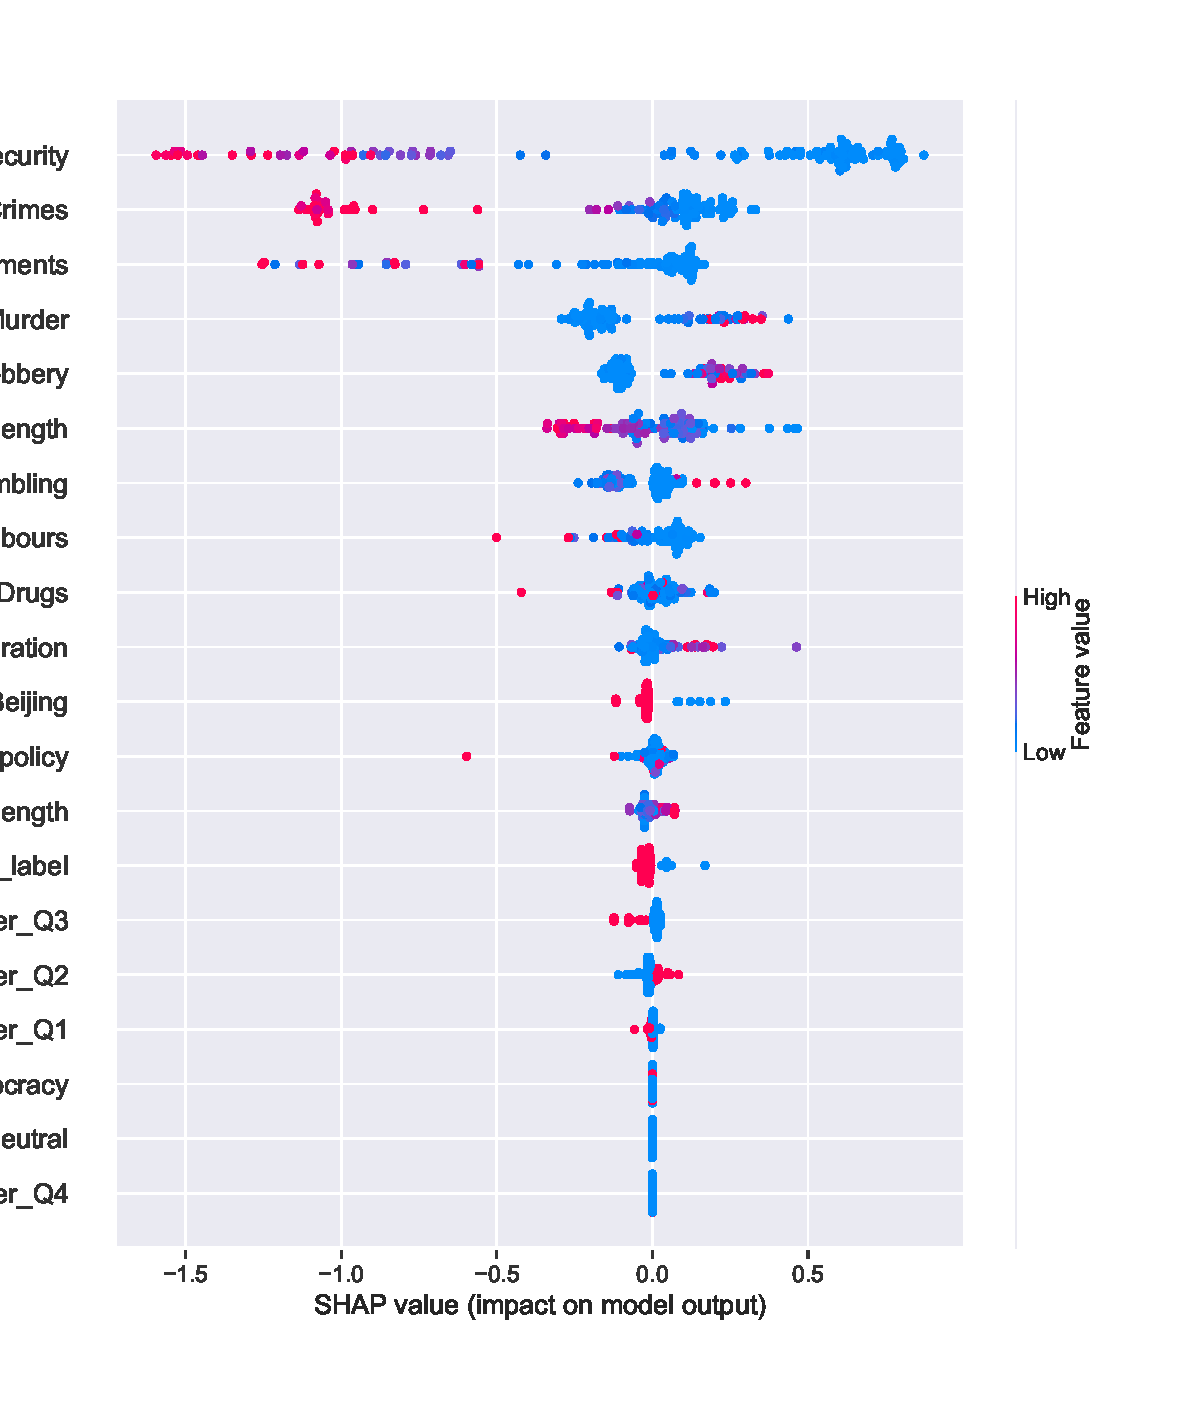
\includegraphics{versions/Chin_Chapter_4_2022-01-10_files/figure-latex/unnamed-chunk-15-5.pdf}

\begin{Shaded}
\begin{Highlighting}[]
\NormalTok{plot\_shap\_values(}\DecValTok{2}\NormalTok{)}
\end{Highlighting}
\end{Shaded}

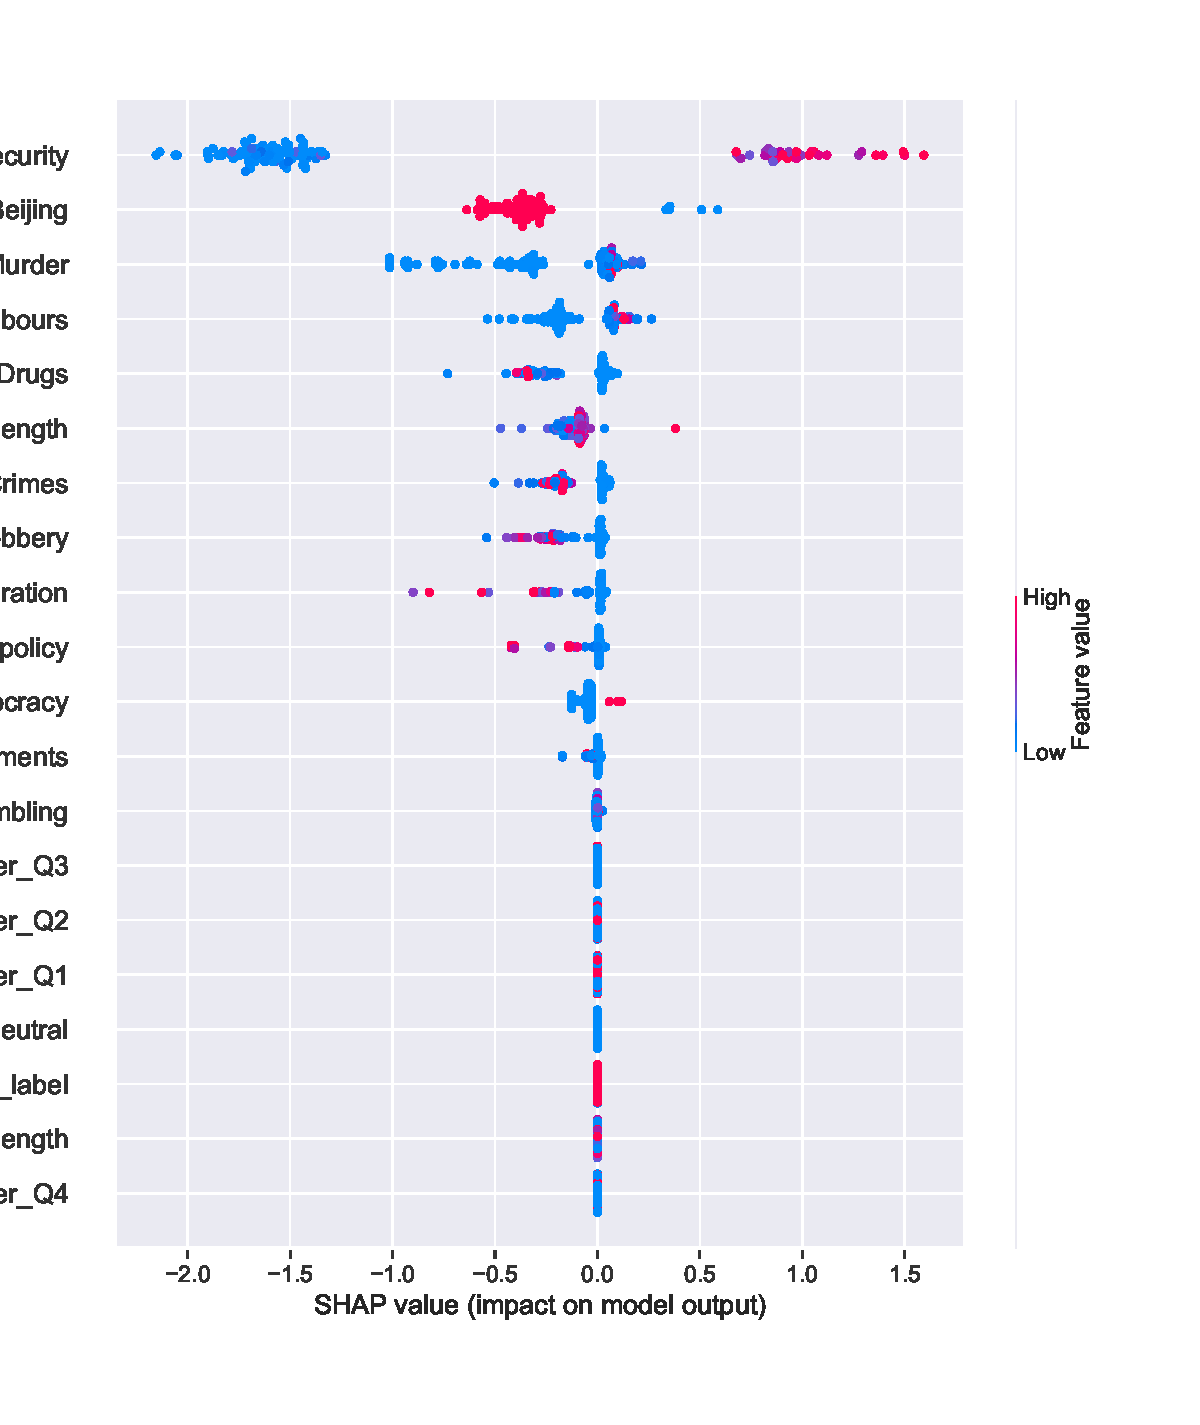
\includegraphics{versions/Chin_Chapter_4_2022-01-10_files/figure-latex/unnamed-chunk-16-7.pdf}

Based on the SHAP values of the features as shown in figures 4.6-4.9, we
can therefore conclude that H\textsubscript{1} is supported by the
evidence produced from the above sentiment analysis on the articles
about asylum seekers in Hong Kong in 2019. Specifically, pro-Beijing
Media outlets are more likely to frame asylum seekers negatively by
using incorrect terms such as ``fake refuges'' to refer to this group of
population or criticising them as social ills, and these media outlets
are quite unlikely to have favourable reportage on non-refoulement
claimants.

Here are also some notable observations about other features in the
dataset. For starters,

\setcounter{chapter}{4}

\hypertarget{conclusion}{%
\chapter{Conclusion}\label{conclusion}}

In conclusion, it is found that at least in 2019, the political camp of
media outlets was associated with their attitudes towards asylum seekers
in Hong Kong. Specifically,

\hypertarget{how-might-the-instigation-of-the-national-security-law-affect-the-public-discourse-on-asylum-seekers-in-hong-kong}{%
\section{How might the instigation of the National Security Law affect
the public discourse on asylum seekers in Hong
Kong?}\label{how-might-the-instigation-of-the-national-security-law-affect-the-public-discourse-on-asylum-seekers-in-hong-kong}}

Just a year after the anti-extradition law protest had started and once
again mobilised a huge section of Hong Kong's society to oppose , the
HKSAR Government promulgated the National Security Law in July 2020
which

As mentioned before, the opposition's political influence has been
greatly crippled since the promulgation of the National Security Law in
July 2020. With the conclusion of the recent 2021 Legislative Council
election after an overhaul of the electoral system which essentially
gatekeeps candidacy only to the ``patriots''
(\protect\hyperlink{ref-lauPatriotsOnlyHong2021}{Lau and Yam 2021}),
Hong Kong's legislature, once a political venue where opposition parties
could access political resources and advocate alternative policy
discourses,

Even in the media

Alternative media such as Apple Daily and Stand News were also forced to
shut down in 2021 due to the

\hypertarget{appendix-the-echoes-of-the-code}{%
\chapter*{Appendix: The Echoes of the
Code}\label{appendix-the-echoes-of-the-code}}
\addcontentsline{toc}{chapter}{Appendix: The Echoes of the Code}

Placeholder

\markboth{References}{References}

\hypertarget{refs}{}
\begin{CSLReferences}{1}{0}
\leavevmode\vadjust pre{\hypertarget{ref-lauPatriotsOnlyHong2021}{}}%
Lau, Jessie, and Shui-yin Sharon Yam. 2021. {``{`{Patriots Only}'}:
{Hong Kong}'s {New Election System} in {Action}.''} \emph{The Diplomat}.
https://thediplomat.com/2021/11/patriots-only-hong-kongs-new-election-system-in-action/.

\leavevmode\vadjust pre{\hypertarget{ref-lundbergSlundbergShap2022}{}}%
Lundberg, Scott. 2022. {``Slundberg/Shap.''}

\leavevmode\vadjust pre{\hypertarget{ref-ngFramingIssueAsylum2019}{}}%
Ng, Isabella, Sharice Fungyee Choi, and Alex Lihshing Chan. 2019.
{``Framing the {Issue} of {Asylum Seekers} and {Refugees} for {Tougher
Refugee Policy}\textemdash a {Study} of the {Media}'s {Portrayal} in
{Post-colonial Hong Kong}.''} \emph{Journal of International Migration
and Integration} 20 (2): 593--617.
\url{https://doi.org/10.1007/s12134-018-0624-7}.

\leavevmode\vadjust pre{\hypertarget{ref-stevensExploringTopicCoherence2012}{}}%
Stevens, Keith, Philip Kegelmeyer, David Andrzejewski, and David
Buttler. 2012. {``Exploring Topic Coherence over Many Models and Many
Topics.''} In \emph{Proceedings of the 2012 Joint Conference on
Empirical Methods in Natural Language Processing and Computational
Natural Language Learning}, 952--61.

\end{CSLReferences}


%%%%% REFERENCES

% JEM: Quote for the top of references (just like a chapter quote if you're using them).  Comment to skip.
% \begin{savequote}[8cm]
% The first kind of intellectual and artistic personality belongs to the hedgehogs, the second to the foxes \dots
%   \qauthor{--- Sir Isaiah Berlin \cite{berlin_hedgehog_2013}}
% \end{savequote}

% \setlength{\baselineskip}{0pt} % JEM: Single-space References
% 
% {\renewcommand*\MakeUppercase[1]{#1}%
% \printbibliography[heading=bibintoc,title={References}]}

\end{document}